After the protocol design phase (Chapter \ref{ch:protocol}) and the implementation with the simulator (Chapter \ref{ch:implementation}), the next step
is to evaluate the different approaches. As the primary goal of this thesis is to provide protection and resilience against malicious routers within
the \gls{noc}, the protocols were tested with varying attacker positions, attack probabilities, and routing strategies. The quality of a scheme
is determined through several metrics that indicate its performance for a given scenario, which are explained below.

The next section establishes notations and key terms that are used throughout this chapter. Afterwards, the environment and frame conditions for the
simulations are delineated (Section \ref{sec:environmenteval}). Following this, the employed attacker model is discussed (Section
\ref{sec:attackermodeleval}) and the configurable parameters for the simulations are explained (Section \ref{sec:configurations}). Subsequently,
the hyperparameters\footnote{The term \textit{hyperparameters} refers to those parameters whose value is determined through a number of preliminary
experiments and remains static for the main experiments.} are fixed through a series of representative experiments (Section
\ref{sec:hyperparamseval}), followed by the main evaluation where the different protocol variants and routing strategies are compared (Section
\ref{sec:perfcompeval}).

\section{Notation}\label{sec:notationeval}
To improve readability, abbreviations are introduced for the protocol variants and network coding modes. This facilitates their representation within
charts, diagrams, and tables.
\begin{itemize}
    \item \textbf{\Gls{ida}} stands for the \textit{individual authentication} protocol version,
    \item \textbf{\Gls{iwa}} represents the \textit{interwoven authentication} approach,
    \item \textbf{\Gls{fga}} denotes the \textit{full-generation authentication} variant,
    \item \textbf{UC} is short for \textit{uncoded}, i.e., the lack of network coding, and
    \item \textbf{G2C3} and \textbf{G2C4} are used for the two network coding variants that were explained in Section \ref{sec:designnc}.
\end{itemize}

These short forms are often combined with a routing strategy when the setup of an experiment is described. For instance, \gls{ida}-UC-\gls{dor} stands for uncoded
individual authentication using dimension order routing.

The term \textit{source flit} is used to refer to flits created by the processing elements before they are handled by the sender's network interface.
Consequently, the combinations obtained by network coding or \gls{mac} flits are not encompassed by this term. In the receiver's network interface,
the source flits are reconstructed by decoding, decrypting and verifying the incoming flits. Network interfaces only forward source flits towards
their local processing elements.

\section{Environment}\label{sec:environmenteval}
The simulator has a variety of input parameters that can be altered to influence its behavior and consequently the outcome of the simulations.
In this section, the parameters that are fixed for all conducted simulations are elaborated, such as flit generation patterns and simulation runtime. Table
\vref{tab:fixedparams} provides a concise overview of these parameters and their values.

\begin{table}
    \centering
    \begin{tabulary}{\textwidth}{L|L}
        Parameter name & Value \\\hline
        \Gls{noc} dimensions & 8x8 (2D mesh) \\
        Clock frequency & 500 MHz \\
        Simulation runtime & \num{50000} cycles \\
        Warmup/cooldown time & 500 cycles \\
        Base network injection rate & 0.2 \\
        Flit destination selection & uniform random \\
        Pair generation & yes \\
    \end{tabulary}
    \caption[Static input parameters for all simulations]{The static, invariant input parameters of the simulator that are used across all
    experiments.}
    \label{tab:fixedparams}
\end{table}

When a simulation is executed, the first 500 cycles are considered warmup time. During this period, no statistics are recorded. This ensures that the
network is in a steady state and already saturated with flits once the recording starts. It is followed by the main simulation of \num{50000}
cycles where statistics are recorded normally. Finally, there are another 500 cooldown cycles at the end. They were appended to ensure that source flits
generated shortly before the end of the main simulation are not classified as lost flits simply because they were not granted enough time to reach their
destination. Thus, source flits generated during the main simulation and arriving at processing elements during the cooldown period are considered
successfully transmitted, while those generated during cooldown are not included in the statistics.

The base network injection rate describes the average number of flits injected into the network per clock cycle at each node, excluding \gls{arq}
flits and retransmissions. The creation rate of flits at the processing elements is adjusted accordingly for each protocol variant to keep the
injection rate constant. For instance, with \gls{ida}-G2C3, every source flit created at a particular processing element results in three flits
injected into the network due to network coding and the additional \gls{mac} flits.

The processing elements create source flits independently from each other. Furthermore, all processing elements use the same creation rate. The
selection of the flits' destinations is performed randomly over all network nodes (excluding the sender's own node). This ensures a uniform
distribution of sources and destinations across the \gls{noc}.

To allow for a fair comparison of the protocol versions, flits are always generated in pairs. This means that when a particular processing
element creates a flit, another one with the same destination is guaranteed to be created on the next clock cycle. This prevents long periods of
buffering for network coded \gls{ida} and \gls{fga} in the sender's network interface: with a pair of flits, a generation can be formed immediately.
This creation pattern is a realistic assumption as in practical applications, flits are usually generated from breaking a data packet down into
smaller parts (cf. Section \ref{sec:flitsfun}). These flits would then depart from the processing element consecutively and have the same
destination. The creation rate of flits is adjusted accordingly to reflect this pattern: for example, with \gls{ida}-G2C3, the probability to create a
pair would be set to $\frac{0.2}{6}$ to preserve the desired base network injection rate of 0.2. Table \vref{tab:creationrates} summarizes the
creation rates for all protocol variants.

\begin{table}
    \centering
    \bgroup
    \renewcommand{\arraystretch}{1.1}
    \begin{tabulary}{\textwidth}{C|C|C}
        Protocol       & Ratio pair : injected & Pair creation rate            \\\hline
        \gls{ida}-UC   & 1:4                   & $\frac{0.2}{4} = 0.05$        \\
        \gls{ida}-G2C3 & 1:6                   & $\frac{0.2}{6} \approx 0.033$ \\
        \gls{ida}-G2C4 & 1:8                   & $\frac{0.2}{8} = 0.025$       \\
        \gls{iwa}-UC   & 1:4                   & $\frac{0.2}{4} = 0.05$        \\
        \gls{iwa}-G2C3 & 1:6                   & $\frac{0.2}{6} \approx 0.033$ \\
        \gls{iwa}-G2C4 & 1:8                   & $\frac{0.2}{8} = 0.025$       \\
        \gls{fga}-G2C3 & 1:4                   & $\frac{0.2}{4} = 0.05$        \\
        \gls{fga}-G2C4 & 1:5                   & $\frac{0.2}{5} = 0.04$
    \end{tabulary}
    \egroup
    \caption[Creation rates of all protocol variants]{The source flit pair creation rates for all protocol variants. The second column displays the
    ratio of one generated source flit pair to the number of flits injected into the network resulting from this pair (excluding potential
    \glspl{arq} and retransmissions). The third column depicts the creation rates as they are adjusted to keep the base network injection rate
    at 0.2 across all variants.}
    \label{tab:creationrates}
\end{table}

Some of the parameters were adopted from the simulation setup that \citeauthor{moriam18activeattackers} \cite{moriam18activeattackers} have employed
in their experiments to render results comparable with their evaluations. These parameters include the \gls{noc} dimensions, the base network
injection rate, and the simulation runtime. The rationale for a clock speed of 500 MHz was outlined in Section \ref{subsec:clockfrequency}.

\section{Attacker Model}\label{sec:attackermodeleval}
As outlined in Section \ref{sec:attackermodelover}, the routers of the \gls{noc} are untrusted components that may be infected by a hardware trojan.
Such a compromised router has the capability to eavesdrop on the communication passing through it (passive attacker) and to maliciously drop or modify
flits (active attacker)\footnote{Routers are also able to inject arbitrary flits into the network to attempt a \gls{dos} attack through bandwidth
depletion. However, this is beyond the scope of this thesis and thus not considered here.}. Protection against an eavesdropper obtaining confidential
information is achieved through the employed encryption, so the remainder of this chapter focuses on the effects of active attacks.

For this thesis, eight of the routers are assumed to be infected, while the remaining ones operate normally. The rationale for not considering all
routers to be infected is that the presence of a hardware trojan entails a higher area occupation of the router due to the additional logic. If all
routers were malicious, it might drive the overall area requirement of the \gls{noc} to suspiciously high values, undermining the adversary's desire
to stay concealed (cf. Section \ref{sec:hardwaretrojans}).

The infected routers are assumed to not mount intelligent attacks, such as only compromising flits from a specific source. Rather, they randomly
attack passing flits based on their \textit{attack probability}. In such an event, the flit is either modified or completely dropped, with both cases
being equiprobable.

For the experiments, the eight infected routers were randomly selected from the 64 network nodes. To obviate large deviations of the recorded
statistics from the average due to their particular distribution, the main experiments were conducted for three different sets of attackers with the
results averaged over them\footnote{This is denoted by \enquote{all} in Table \ref{tab:inputparams} and subsequent experiment setup descriptions.}.
Figure \vref{fig:attackerpositions} illustrates the three selected distributions.

\begin{figure}
    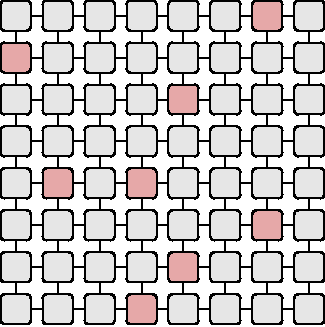
\includegraphics[width=0.3\textwidth]{attacker-positions-1}\hfill
    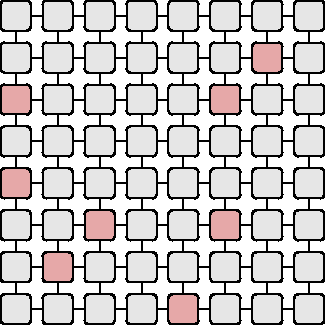
\includegraphics[width=0.3\textwidth]{attacker-positions-2}\hfill
    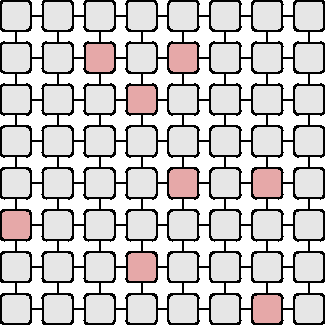
\includegraphics[width=0.3\textwidth]{attacker-positions-3}
    \caption[Malicious router distributions]{The three distributions of 8 malicious routers over the 8x8 \gls{noc} that were used in experiments.}
    \label{fig:attackerpositions}
\end{figure}

\section{Configurations}\label{sec:configurations}
In addition to the static input parameters presented in Section \ref{sec:environmenteval}, there are several variable ones that constitute the setup
of an experiment. Naturally, they include the protocol variant and the routing strategy, but are not limited to those. Table \vref{tab:inputparams}
lists all the variable input parameters.

\begin{table}
    \centering
    \begin{tabulary}{\textwidth}{C|C|C}
        Parameter name & Value range & Placeholder \\\hline
        Protocol variant & $\{\text{\gls{ida}}, \text{\gls{iwa}}, \text{\gls{fga}}\}$ & \pProtVar{} \\
        Network coding & $\{\text{UC}, \text{G2C3}, \text{G2C4}\}$ & \pNCMode{} \\
        Routing strategy & $\{\text{\gls{dor}}, \text{\gls{dm}}, \text{\gls{romm}}, \text{\gls{ramm}}\}$ & \pRStrat{} \\
        No. of encryption modules & $\mathbb{N}^*$ & \pEncMods{} \\
        No. of authentication modules & $\mathbb{N}^*$ & \pAuthMods{} \\
        \Gls{arq} limit & $\{1, 2\}$ & \pARQLimit{} \\
        \Gls{arq} timeout in cycles & $\mathbb{N}^*$ & \pARQTimeout{} \\
        Port queue size in flits & $\mathbb{N}^* \cup \infty$ & \pRQSize{} \\
        Set of attackers & $\{1, 2, 3, \text{all}, \text{none}\}$ & \pAttackerSet{} \\
        Attack probability & $[0, 0.5]$ & \pAttackProb{} \\
    \end{tabulary}
    \caption[Variable input parameters for the simulations]{The variable input parameters for the simulations. The third column shows the placeholders
    that are used in subsequent experiment setups to represent the corresponding parameters.}
    \label{tab:inputparams}
\end{table}

Each network interface contains a number of encryption and authentication modules. On the one hand, there need to be enough modules to process both
departing and arriving flits quickly without incurring congestions. On the other hand, each additional module entails a higher area requirement for
the network interfaces. Thus, a reasonable trade-off between latency and area needs to be determined. This hyperparameter is examined in Section
\ref{subsec:numcryptomodules}.

The \gls{arq} limit is the number of \glspl{arq} that are allowed to be issued per transmission unit (see Section \ref{subsec:arqretransmissions}).
Only the values 1 and 2 are considered here for multiple reasons. First, the more \glspl{arq} are allowed, the larger the \glspl{rtb} need to be:
since additional \glspl{arq} are only sent if the preceding ones did not yield successful retransmissions, senders need to retain flits in their
\glspl{rtb} over a longer period. Second, if more \glspl{arq} and consequently more retransmissions are injected into the network, congestions become
more likely, which in turn may induce timeouts for other transmissions.

The value of the \gls{arq} timeout is the first hyperparameter that is fixed through an experiment (Section \ref{subsec:arqtimeouts}). As explained in
Section \ref{subsec:arqretransmissions}, it represents the amount of clock cycles after receiving a flit from a particular transmission unit until the
remainder of this unit is considered lost.

The sizes of the port queues of the routers are another hyperparameter. Unfortunately, it could only be determined for \gls{dor}. The absence of
virtual channels in the routers (cf. Section \ref{subsec:singlecyclerouting}) incurs deadlocks for the other routing strategies if a limited queue
size is enforced. For instance, \gls{romm} routing necessitates two virtual channels (one for each phase) to guarantee deadlock freedom
\cite[4]{nesson95romm}. \Gls{dor}, however, is not affected by deadlocks, even without virtual channels \cite[9]{ni93routingsurvey}. Thus, as a
workaround, a hard queue size limit is only implemented for \gls{dor}\footnote{With a hard queue size limit, routers must delay flits that are
to be sent via a congested link, as they would be discarded otherwise.}. For the other strategies, congestion signals are still sent out once a queue
has reached the given size, but it will continue to accept incoming flits. While \gls{romm}, being oblivious, ignores these signals, \gls{dm} and
\gls{ramm} attempt to avoid congested links as much as possible. In Section \ref{subsec:portqueuesizes}, the experiment to determine the size limit
for \gls{dor} is described.

Finally, the properties of the attacking routers may be configured via the set of attackers and their attack probability. The set of attackers refers
to one of the three sets described in Figure \ref{fig:attackerpositions}. A value of \textit{all} indicates that the experiments were conducted for
each of the sets independently and the results are averaged across the three settings. If no attackers are present, \textit{none} is used. The attack
probability parameter defines the likelihood for a malicious router to attack a flit as described above (Section \ref{sec:attackermodeleval}).

\section{Determining The Hyperparameters}\label{sec:hyperparamseval}
\subsection{ARQ Timeouts}\label{subsec:arqtimeouts}
The first hyperparameter that is fixed through an experiment is the number of cycles for an \gls{arq} timeout. In Section
\ref{subsec:arqretransmissions}, it was mentioned that two different timeout values exist: in addition to the inter-arrival timeout, there is another,
higher value that is used after an \gls{arq} was issued to await the answer (the post-\gls{arq} timeout). However, only the former
is empirically determined, while the latter is calculated from the inter-arrival timeout, the Manhattan distance between the
two affected communication partners, and the \gls{rtb} lookup time. More precisely, if $t_1$ is the inter-arrival timeout, $t_2(S, D)$ is the post-\gls{arq} timeout for a
particular source $S$ and destination $D$, $d$ is the Manhattan distance between the two nodes, and $l$ is the \gls{rtb} lookup time, then $t_2(S, D)
= t_1 + 2d + l$. Figure \vref{fig:arqtimeoutscalc} illustrates this calculation. 

\begin{figure}
    \centering
    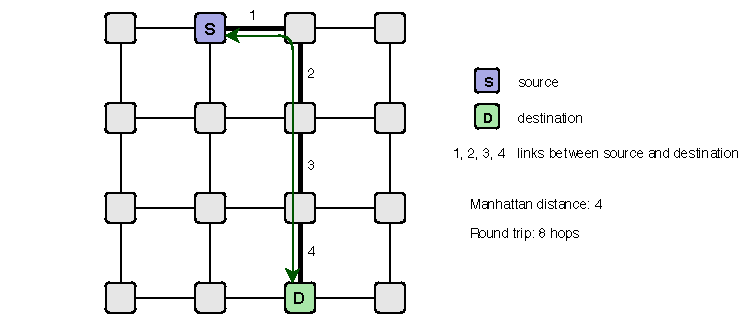
\includegraphics[width=0.9\textwidth]{arq-timeouts-calc}
    \caption[Example of ARQ timeout calculation]{Example for the calculation of \gls{arq} timeouts. With a Manhattan distance of 4 between source $S$ and
    destination $D$ and a given inter-arrival timeout $t_1$, the \gls{arq} timeout $t_2(S, D)$ is computed as $t_1 + 2 \cdot 4 = t_1 + 8$ cycles.}
    \label{fig:arqtimeoutscalc}
\end{figure}

Thus, the purpose of this experiment is to determine a suitable value for $t_1$. The idea is that in a network devoid of attackers, ideally no
\glspl{arq} are issued since no flits are lost. However, due to random deviations from the average flit injection rate, the network load varies over
time and congestions in some routers
may occur. The resulting increased transmission delays may be high enough to trigger timeouts even when an \gls{arq} is not necessary. Sporadic
occurances of such cases cannot be ruled out, but should rarely happen. However, simply increasing the timeout until these cases vanish is undesirable
for two reasons. First, a high timeout directly corresponds to high latencies when flit losses necessitate \glspl{arq}. Second, the later an \gls{arq}
is issued, the larger the \gls{rtb} of the communication partner needs to be so that the flits in question are not already overwritten when the
\gls{arq} arrives. The goal of this experiment is to find a reasonable middle ground: the smallest timeout that does not entail a significant number of
unnecessary \glspl{arq} will be used for the subsequent evaluations.

\begin{table}
    \centering
    \begin{tabulary}{\textwidth}{C|C|C|C|C|C|C|C|C|C}
        \pProtVar{} & \pNCMode{} & \pEncMods{} & \pAuthMods{} & \pRQSize{} & \pARQLimit{} & \pARQTimeout{} & \pRStrat{} & \pAttackerSet{} & \pAttackProb{} \\\hline
        \gls{ida}   & varying    & 5           & 15           & unlimited  & 1            & varying        & \gls{dor}  & none            & 0              \\
    \end{tabulary}
    \caption[Input parameters for ARQ timeouts experiment]{The input parameters for the simulator in the \gls{arq} timeouts experiment.}
    \label{tab:setuparqtimeouts}
\end{table}

Since $t_1$ is the first parameter to be fixed, the other input values for the simulation are estimates. They are summarized in Table
\vref{tab:setuparqtimeouts}. The tests are for the most part independent of the protocol variant as the same injection rate is used for all of them.
Hence, \gls{ida} was selected as it features the largest variety of transmission unit sizes (from 2 for UC up to 8 for G2C4) and all \glspl{arq} are
issued per transmission unit. The number of crypto modules was set to a sufficiently high value to ensure that no congestions occur inside the network
interfaces. Similarly, the router port queue sizes are not limited as no fitting value was determined yet. \Gls{dor} is employed since it is used as
the baseline for all experiments before evaluating the effects of other routing strategies.

\begin{figure}
    \centering
    % GNUPLOT: LaTeX picture with Postscript
\begingroup
\newcommand{\ft}[0]{\footnotesize}
  \makeatletter
  \providecommand\color[2][]{%
    \GenericError{(gnuplot) \space\space\space\@spaces}{%
      Package color not loaded in conjunction with
      terminal option `colourtext'%
    }{See the gnuplot documentation for explanation.%
    }{Either use 'blacktext' in gnuplot or load the package
      color.sty in LaTeX.}%
    \renewcommand\color[2][]{}%
  }%
  \providecommand\includegraphics[2][]{%
    \GenericError{(gnuplot) \space\space\space\@spaces}{%
      Package graphicx or graphics not loaded%
    }{See the gnuplot documentation for explanation.%
    }{The gnuplot epslatex terminal needs graphicx.sty or graphics.sty.}%
    \renewcommand\includegraphics[2][]{}%
  }%
  \providecommand\rotatebox[2]{#2}%
  \@ifundefined{ifGPcolor}{%
    \newif\ifGPcolor
    \GPcolortrue
  }{}%
  \@ifundefined{ifGPblacktext}{%
    \newif\ifGPblacktext
    \GPblacktextfalse
  }{}%
  % define a \g@addto@macro without @ in the name:
  \let\gplgaddtomacro\g@addto@macro
  % define empty templates for all commands taking text:
  \gdef\gplbacktext{}%
  \gdef\gplfronttext{}%
  \makeatother
  \ifGPblacktext
    % no textcolor at all
    \def\colorrgb#1{}%
    \def\colorgray#1{}%
  \else
    % gray or color?
    \ifGPcolor
      \def\colorrgb#1{\color[rgb]{#1}}%
      \def\colorgray#1{\color[gray]{#1}}%
      \expandafter\def\csname LTw\endcsname{\color{white}}%
      \expandafter\def\csname LTb\endcsname{\color{black}}%
      \expandafter\def\csname LTa\endcsname{\color{black}}%
      \expandafter\def\csname LT0\endcsname{\color[rgb]{1,0,0}}%
      \expandafter\def\csname LT1\endcsname{\color[rgb]{0,1,0}}%
      \expandafter\def\csname LT2\endcsname{\color[rgb]{0,0,1}}%
      \expandafter\def\csname LT3\endcsname{\color[rgb]{1,0,1}}%
      \expandafter\def\csname LT4\endcsname{\color[rgb]{0,1,1}}%
      \expandafter\def\csname LT5\endcsname{\color[rgb]{1,1,0}}%
      \expandafter\def\csname LT6\endcsname{\color[rgb]{0,0,0}}%
      \expandafter\def\csname LT7\endcsname{\color[rgb]{1,0.3,0}}%
      \expandafter\def\csname LT8\endcsname{\color[rgb]{0.5,0.5,0.5}}%
    \else
      % gray
      \def\colorrgb#1{\color{black}}%
      \def\colorgray#1{\color[gray]{#1}}%
      \expandafter\def\csname LTw\endcsname{\color{white}}%
      \expandafter\def\csname LTb\endcsname{\color{black}}%
      \expandafter\def\csname LTa\endcsname{\color{black}}%
      \expandafter\def\csname LT0\endcsname{\color{black}}%
      \expandafter\def\csname LT1\endcsname{\color{black}}%
      \expandafter\def\csname LT2\endcsname{\color{black}}%
      \expandafter\def\csname LT3\endcsname{\color{black}}%
      \expandafter\def\csname LT4\endcsname{\color{black}}%
      \expandafter\def\csname LT5\endcsname{\color{black}}%
      \expandafter\def\csname LT6\endcsname{\color{black}}%
      \expandafter\def\csname LT7\endcsname{\color{black}}%
      \expandafter\def\csname LT8\endcsname{\color{black}}%
    \fi
  \fi
    \setlength{\unitlength}{0.0500bp}%
    \ifx\gptboxheight\undefined%
      \newlength{\gptboxheight}%
      \newlength{\gptboxwidth}%
      \newsavebox{\gptboxtext}%
    \fi%
    \setlength{\fboxrule}{0.5pt}%
    \setlength{\fboxsep}{1pt}%
\begin{picture}(7920.00,3600.00)%
    \gplgaddtomacro\gplbacktext{%
      \csname LTb\endcsname%
      \put(946,704){\makebox(0,0)[r]{\strut{}$0$}}%
      \put(946,1230){\makebox(0,0)[r]{\strut{}$0.05$}}%
      \put(946,1756){\makebox(0,0)[r]{\strut{}$0.1$}}%
      \put(946,2283){\makebox(0,0)[r]{\strut{}$0.15$}}%
      \put(946,2809){\makebox(0,0)[r]{\strut{}$0.2$}}%
      \put(946,3335){\makebox(0,0)[r]{\strut{}$0.25$}}%
      \put(1615,484){\makebox(0,0){\strut{}$4$}}%
      \put(2689,484){\makebox(0,0){\strut{}$6$}}%
      \put(3763,484){\makebox(0,0){\strut{}$8$}}%
      \put(4838,484){\makebox(0,0){\strut{}$10$}}%
      \put(5912,484){\makebox(0,0){\strut{}$12$}}%
      \put(6986,484){\makebox(0,0){\strut{}$14$}}%
    }%
    \gplgaddtomacro\gplfronttext{%
      \csname LTb\endcsname%
      \put(176,2019){\rotatebox{-270}{\makebox(0,0){\strut{}\ft ARQs per source flit}}}%
      \put(4300,154){\makebox(0,0){\strut{}\ft Timeout in cycles}}%
      \csname LTb\endcsname%
      \put(6788,3197){\makebox(0,0)[r]{\strut{}\ft UC}}%
      \csname LTb\endcsname%
      \put(6788,3047){\makebox(0,0)[r]{\strut{}\ft G2C3}}%
      \csname LTb\endcsname%
      \put(6788,2897){\makebox(0,0)[r]{\strut{}\ft G2C4}}%
    }%
    \gplbacktext
    \put(0,0){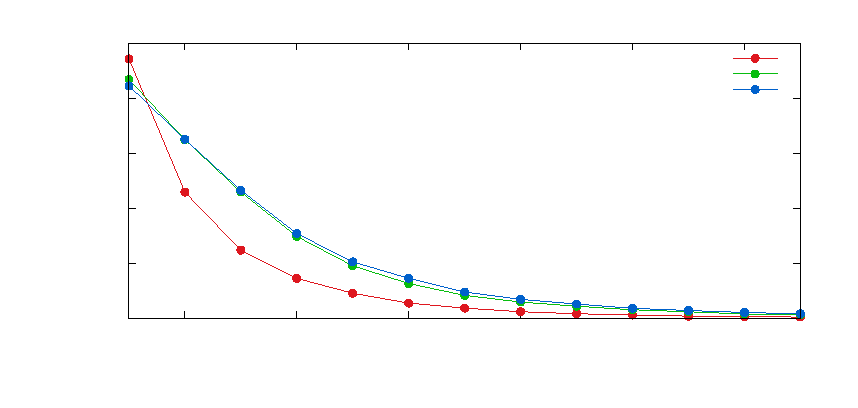
\includegraphics{../plots/arqtimeouts}}%
    \gplfronttext
  \end{picture}%
\endgroup

    \caption[Results for ARQ timeouts experiment]{long}
    \label{fig:resultsarqtimeouts}
\end{figure}

Figure \vref{fig:resultsarqtimeouts} presents the number of \glspl{arq} issued for $t_1 \in [3, 15]$ clock cycles. The values are shown in relation to
the number of created source flits instead of the number of transmission units as the size of the latter varies significantly depending on the network
coding scheme. For timeout values of 12 or greater, less than 1 \gls{arq} per 100 source flits is sent, which is considered sufficiently small here.
Hence, $t_1 = 12$ is chosen and used in all future experiments.

% TODO: Use sadias formula for RTB size estimation

\subsection{Number Of Crypto Modules}\label{subsec:numcryptomodules}
The second experiment concerns itself with the number of required encryption and authentication modules in the network interfaces. Here, a
reasonable trade-off between occupied chip area and performance needs to be determined: there should be just enough modules to keep the waiting time
of flits for a free module low.

In Figure \ref{fig:omnetni}, it was shown that the flits from four queues compete for access: two for encryption modules and two for authentication
modules. The idea of this experiment is to measure the time (in clock cycles) that flits are enqueued before they are granted access to a crypto
module. In addition to the average, the maximum queue time was investigated as well to take periods of increased network traffic into account. Even
during such periods, the flits should not suffer unreasonably high delays.

\begin{table}
    \centering
    \begin{tabulary}{\textwidth}{C|C|C|C|C|C|C|C|C|C}
        \pProtVar{} & \pNCMode{} & \pEncMods{} & \pAuthMods{} & \pRQSize{} & \pARQLimit{} & \pARQTimeout{} & \pRStrat{} & \pAttackerSet{} & \pAttackProb{} \\\hline
        varying     & varying    & varying     & varying      & unlimited  & 1            & 12             & \gls{dor}  & 1               & 0.2            \\
    \end{tabulary}
    \caption[Input parameters for number of crypto modules experiment]{The input parameters for the simulator in the experiment to determine the
    number of required crypto modules.}
    \label{tab:setupnumcrypto}
\end{table}

Table \vref{tab:setupnumcrypto} shows the input parameters used for this experiment. Since the internal structure of the network interfaces and the
number of cycles for authentication vary considerably depending on the protocol variant, all of them were investigated and compared. The rationale for
unlimited router port queue sizes is the same as in the \gls{arq} timeout experiment (see above). The \gls{arq} limit is set to 1 for the same reason
that \gls{dor} is used as the routing strategy: they are baseline values for all experiments until the effects of varying them are investigated later
on. The \gls{arq} timeout is set to 12, which is the value identified in the previous experiment (Section \ref{subsec:arqtimeouts}). Attackers
with a medium attack probability are added as their presence entails an increase in required decryptions and \gls{mac} computations: if an integrity
breach is detected, both these actions need to be executed for the subsequent retransmissions as well.

The minimum waiting time of a flit is one cycle: as the queues provide synchronization with the global clock, even flits that arrive at an empty queue
can be sent out at the earliest on the next clock tick. Furthermore, the fact that at most one flit can be sent out from a queue per cycle induces an
upper bound on the number of required crypto modules. For encryption, four modules always suffice as processing a flit takes two cycles and at most two
flits can be distributed among the modules per cycle (one from the encryption and one from the decryption queue). The upper bound for authentication
modules is calculated in the same manner, but depends on the protocol variant. For \gls{ida} and \gls{iwa}, it is 12 and 10 modules, respectively, as
the authentication process requires six and five cycles, respectively. \Gls{fga} operates slightly differently because two flits are required for a
single authentication procedure. Thus, an authentication module is busy for 11 cycles (one to wait for the second flit, then 10 for the \gls{mac}
computation). Hence, at most 11 modules are required for this variant.

\begin{figure}
    \centering
    \begin{tabular}{ll}
        % GNUPLOT: LaTeX picture with Postscript
\begingroup
\newcommand{\ft}[0]{\footnotesize}\newcommand{\ty}[0]{\tiny}
  \makeatletter
  \providecommand\color[2][]{%
    \GenericError{(gnuplot) \space\space\space\@spaces}{%
      Package color not loaded in conjunction with
      terminal option `colourtext'%
    }{See the gnuplot documentation for explanation.%
    }{Either use 'blacktext' in gnuplot or load the package
      color.sty in LaTeX.}%
    \renewcommand\color[2][]{}%
  }%
  \providecommand\includegraphics[2][]{%
    \GenericError{(gnuplot) \space\space\space\@spaces}{%
      Package graphicx or graphics not loaded%
    }{See the gnuplot documentation for explanation.%
    }{The gnuplot epslatex terminal needs graphicx.sty or graphics.sty.}%
    \renewcommand\includegraphics[2][]{}%
  }%
  \providecommand\rotatebox[2]{#2}%
  \@ifundefined{ifGPcolor}{%
    \newif\ifGPcolor
    \GPcolortrue
  }{}%
  \@ifundefined{ifGPblacktext}{%
    \newif\ifGPblacktext
    \GPblacktextfalse
  }{}%
  % define a \g@addto@macro without @ in the name:
  \let\gplgaddtomacro\g@addto@macro
  % define empty templates for all commands taking text:
  \gdef\gplbacktext{}%
  \gdef\gplfronttext{}%
  \makeatother
  \ifGPblacktext
    % no textcolor at all
    \def\colorrgb#1{}%
    \def\colorgray#1{}%
  \else
    % gray or color?
    \ifGPcolor
      \def\colorrgb#1{\color[rgb]{#1}}%
      \def\colorgray#1{\color[gray]{#1}}%
      \expandafter\def\csname LTw\endcsname{\color{white}}%
      \expandafter\def\csname LTb\endcsname{\color{black}}%
      \expandafter\def\csname LTa\endcsname{\color{black}}%
      \expandafter\def\csname LT0\endcsname{\color[rgb]{1,0,0}}%
      \expandafter\def\csname LT1\endcsname{\color[rgb]{0,1,0}}%
      \expandafter\def\csname LT2\endcsname{\color[rgb]{0,0,1}}%
      \expandafter\def\csname LT3\endcsname{\color[rgb]{1,0,1}}%
      \expandafter\def\csname LT4\endcsname{\color[rgb]{0,1,1}}%
      \expandafter\def\csname LT5\endcsname{\color[rgb]{1,1,0}}%
      \expandafter\def\csname LT6\endcsname{\color[rgb]{0,0,0}}%
      \expandafter\def\csname LT7\endcsname{\color[rgb]{1,0.3,0}}%
      \expandafter\def\csname LT8\endcsname{\color[rgb]{0.5,0.5,0.5}}%
    \else
      % gray
      \def\colorrgb#1{\color{black}}%
      \def\colorgray#1{\color[gray]{#1}}%
      \expandafter\def\csname LTw\endcsname{\color{white}}%
      \expandafter\def\csname LTb\endcsname{\color{black}}%
      \expandafter\def\csname LTa\endcsname{\color{black}}%
      \expandafter\def\csname LT0\endcsname{\color{black}}%
      \expandafter\def\csname LT1\endcsname{\color{black}}%
      \expandafter\def\csname LT2\endcsname{\color{black}}%
      \expandafter\def\csname LT3\endcsname{\color{black}}%
      \expandafter\def\csname LT4\endcsname{\color{black}}%
      \expandafter\def\csname LT5\endcsname{\color{black}}%
      \expandafter\def\csname LT6\endcsname{\color{black}}%
      \expandafter\def\csname LT7\endcsname{\color{black}}%
      \expandafter\def\csname LT8\endcsname{\color{black}}%
    \fi
  \fi
    \setlength{\unitlength}{0.0500bp}%
    \ifx\gptboxheight\undefined%
      \newlength{\gptboxheight}%
      \newlength{\gptboxwidth}%
      \newsavebox{\gptboxtext}%
    \fi%
    \setlength{\fboxrule}{0.5pt}%
    \setlength{\fboxsep}{1pt}%
\begin{picture}(3600.00,3168.00)%
    \gplgaddtomacro\gplbacktext{%
      \csname LTb\endcsname%
      \put(858,660){\makebox(0,0)[r]{\strut{}\ft 1}}%
      \put(858,1782){\makebox(0,0)[r]{\strut{}\ft 10}}%
      \put(858,2903){\makebox(0,0)[r]{\strut{}\ft 100}}%
      \put(990,440){\makebox(0,0){\strut{}\ft 1}}%
      \put(1728,440){\makebox(0,0){\strut{}\ft 2}}%
      \put(2465,440){\makebox(0,0){\strut{}\ft 3}}%
      \put(3203,440){\makebox(0,0){\strut{}\ft 4}}%
    }%
    \gplgaddtomacro\gplfronttext{%
      \csname LTb\endcsname%
      \put(352,1781){\rotatebox{-270}{\makebox(0,0){\strut{}\ft Enqueued time in cycles}}}%
      \put(2096,154){\makebox(0,0){\strut{}\ft No. of encryption modules}}%
      \csname LTb\endcsname%
      \put(2468,2765){\makebox(0,0)[r]{\strut{}\ty IDA-UC max}}%
      \csname LTb\endcsname%
      \put(2468,2615){\makebox(0,0)[r]{\strut{}\ty avg}}%
      \csname LTb\endcsname%
      \put(2468,2465){\makebox(0,0)[r]{\strut{}\ty G2C3 max}}%
      \csname LTb\endcsname%
      \put(2468,2315){\makebox(0,0)[r]{\strut{}\ty avg}}%
      \csname LTb\endcsname%
      \put(2468,2165){\makebox(0,0)[r]{\strut{}\ty G2C4 max}}%
      \csname LTb\endcsname%
      \put(2468,2015){\makebox(0,0)[r]{\strut{}\ty avg}}%
    }%
    \gplbacktext
    \put(0,0){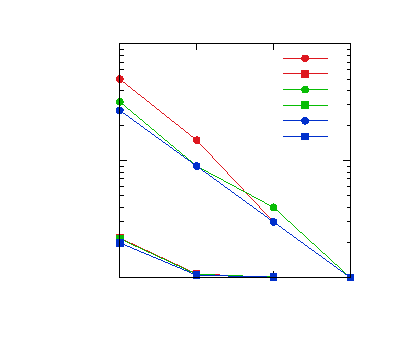
\includegraphics{../plots/encmodules-ida}}%
    \gplfronttext
  \end{picture}%
\endgroup
 & % GNUPLOT: LaTeX picture with Postscript
\begingroup
\newcommand{\ft}[0]{\footnotesize}\newcommand{\ty}[0]{\tiny}
  \makeatletter
  \providecommand\color[2][]{%
    \GenericError{(gnuplot) \space\space\space\@spaces}{%
      Package color not loaded in conjunction with
      terminal option `colourtext'%
    }{See the gnuplot documentation for explanation.%
    }{Either use 'blacktext' in gnuplot or load the package
      color.sty in LaTeX.}%
    \renewcommand\color[2][]{}%
  }%
  \providecommand\includegraphics[2][]{%
    \GenericError{(gnuplot) \space\space\space\@spaces}{%
      Package graphicx or graphics not loaded%
    }{See the gnuplot documentation for explanation.%
    }{The gnuplot epslatex terminal needs graphicx.sty or graphics.sty.}%
    \renewcommand\includegraphics[2][]{}%
  }%
  \providecommand\rotatebox[2]{#2}%
  \@ifundefined{ifGPcolor}{%
    \newif\ifGPcolor
    \GPcolortrue
  }{}%
  \@ifundefined{ifGPblacktext}{%
    \newif\ifGPblacktext
    \GPblacktextfalse
  }{}%
  % define a \g@addto@macro without @ in the name:
  \let\gplgaddtomacro\g@addto@macro
  % define empty templates for all commands taking text:
  \gdef\gplbacktext{}%
  \gdef\gplfronttext{}%
  \makeatother
  \ifGPblacktext
    % no textcolor at all
    \def\colorrgb#1{}%
    \def\colorgray#1{}%
  \else
    % gray or color?
    \ifGPcolor
      \def\colorrgb#1{\color[rgb]{#1}}%
      \def\colorgray#1{\color[gray]{#1}}%
      \expandafter\def\csname LTw\endcsname{\color{white}}%
      \expandafter\def\csname LTb\endcsname{\color{black}}%
      \expandafter\def\csname LTa\endcsname{\color{black}}%
      \expandafter\def\csname LT0\endcsname{\color[rgb]{1,0,0}}%
      \expandafter\def\csname LT1\endcsname{\color[rgb]{0,1,0}}%
      \expandafter\def\csname LT2\endcsname{\color[rgb]{0,0,1}}%
      \expandafter\def\csname LT3\endcsname{\color[rgb]{1,0,1}}%
      \expandafter\def\csname LT4\endcsname{\color[rgb]{0,1,1}}%
      \expandafter\def\csname LT5\endcsname{\color[rgb]{1,1,0}}%
      \expandafter\def\csname LT6\endcsname{\color[rgb]{0,0,0}}%
      \expandafter\def\csname LT7\endcsname{\color[rgb]{1,0.3,0}}%
      \expandafter\def\csname LT8\endcsname{\color[rgb]{0.5,0.5,0.5}}%
    \else
      % gray
      \def\colorrgb#1{\color{black}}%
      \def\colorgray#1{\color[gray]{#1}}%
      \expandafter\def\csname LTw\endcsname{\color{white}}%
      \expandafter\def\csname LTb\endcsname{\color{black}}%
      \expandafter\def\csname LTa\endcsname{\color{black}}%
      \expandafter\def\csname LT0\endcsname{\color{black}}%
      \expandafter\def\csname LT1\endcsname{\color{black}}%
      \expandafter\def\csname LT2\endcsname{\color{black}}%
      \expandafter\def\csname LT3\endcsname{\color{black}}%
      \expandafter\def\csname LT4\endcsname{\color{black}}%
      \expandafter\def\csname LT5\endcsname{\color{black}}%
      \expandafter\def\csname LT6\endcsname{\color{black}}%
      \expandafter\def\csname LT7\endcsname{\color{black}}%
      \expandafter\def\csname LT8\endcsname{\color{black}}%
    \fi
  \fi
    \setlength{\unitlength}{0.0500bp}%
    \ifx\gptboxheight\undefined%
      \newlength{\gptboxheight}%
      \newlength{\gptboxwidth}%
      \newsavebox{\gptboxtext}%
    \fi%
    \setlength{\fboxrule}{0.5pt}%
    \setlength{\fboxsep}{1pt}%
\begin{picture}(4464.00,3168.00)%
    \gplgaddtomacro\gplbacktext{%
      \csname LTb\endcsname%
      \put(858,660){\makebox(0,0)[r]{\strut{}\ft 1}}%
      \put(858,1782){\makebox(0,0)[r]{\strut{}\ft 10}}%
      \put(858,2903){\makebox(0,0)[r]{\strut{}\ft 100}}%
      \put(990,440){\makebox(0,0){\strut{}\ft 1}}%
      \put(1270,440){\makebox(0,0){\strut{}\ft 2}}%
      \put(1549,440){\makebox(0,0){\strut{}\ft 3}}%
      \put(1829,440){\makebox(0,0){\strut{}\ft 4}}%
      \put(2109,440){\makebox(0,0){\strut{}\ft 5}}%
      \put(2389,440){\makebox(0,0){\strut{}\ft 6}}%
      \put(2668,440){\makebox(0,0){\strut{}\ft 7}}%
      \put(2948,440){\makebox(0,0){\strut{}\ft 8}}%
      \put(3228,440){\makebox(0,0){\strut{}\ft 9}}%
      \put(3508,440){\makebox(0,0){\strut{}\ft 10}}%
      \put(3787,440){\makebox(0,0){\strut{}\ft 11}}%
      \put(4067,440){\makebox(0,0){\strut{}\ft 12}}%
    }%
    \gplgaddtomacro\gplfronttext{%
      \csname LTb\endcsname%
      \put(352,1781){\rotatebox{-270}{\makebox(0,0){\strut{}\ft Enqueued time in cycles}}}%
      \put(2528,154){\makebox(0,0){\strut{}\ft No. of authentication modules}}%
      \csname LTb\endcsname%
      \put(3332,2765){\makebox(0,0)[r]{\strut{}\ty IDA-UC max}}%
      \csname LTb\endcsname%
      \put(3332,2615){\makebox(0,0)[r]{\strut{}\ty avg}}%
      \csname LTb\endcsname%
      \put(3332,2465){\makebox(0,0)[r]{\strut{}\ty G2C3 max}}%
      \csname LTb\endcsname%
      \put(3332,2315){\makebox(0,0)[r]{\strut{}\ty avg}}%
      \csname LTb\endcsname%
      \put(3332,2165){\makebox(0,0)[r]{\strut{}\ty G2C4 max}}%
      \csname LTb\endcsname%
      \put(3332,2015){\makebox(0,0)[r]{\strut{}\ty avg}}%
    }%
    \gplbacktext
    \put(0,0){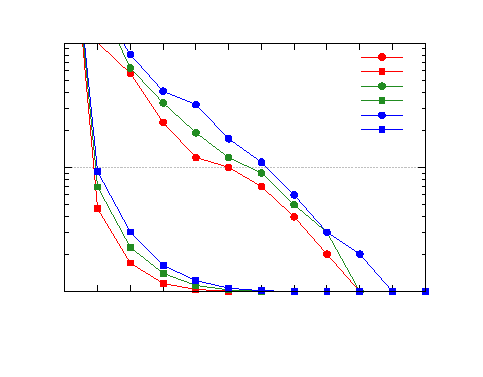
\includegraphics{../plots/authmodules-ida}}%
    \gplfronttext
  \end{picture}%
\endgroup
 \\
        % GNUPLOT: LaTeX picture with Postscript
\begingroup
\newcommand{\ft}[0]{\footnotesize}\newcommand{\ty}[0]{\tiny}
  \makeatletter
  \providecommand\color[2][]{%
    \GenericError{(gnuplot) \space\space\space\@spaces}{%
      Package color not loaded in conjunction with
      terminal option `colourtext'%
    }{See the gnuplot documentation for explanation.%
    }{Either use 'blacktext' in gnuplot or load the package
      color.sty in LaTeX.}%
    \renewcommand\color[2][]{}%
  }%
  \providecommand\includegraphics[2][]{%
    \GenericError{(gnuplot) \space\space\space\@spaces}{%
      Package graphicx or graphics not loaded%
    }{See the gnuplot documentation for explanation.%
    }{The gnuplot epslatex terminal needs graphicx.sty or graphics.sty.}%
    \renewcommand\includegraphics[2][]{}%
  }%
  \providecommand\rotatebox[2]{#2}%
  \@ifundefined{ifGPcolor}{%
    \newif\ifGPcolor
    \GPcolortrue
  }{}%
  \@ifundefined{ifGPblacktext}{%
    \newif\ifGPblacktext
    \GPblacktextfalse
  }{}%
  % define a \g@addto@macro without @ in the name:
  \let\gplgaddtomacro\g@addto@macro
  % define empty templates for all commands taking text:
  \gdef\gplbacktext{}%
  \gdef\gplfronttext{}%
  \makeatother
  \ifGPblacktext
    % no textcolor at all
    \def\colorrgb#1{}%
    \def\colorgray#1{}%
  \else
    % gray or color?
    \ifGPcolor
      \def\colorrgb#1{\color[rgb]{#1}}%
      \def\colorgray#1{\color[gray]{#1}}%
      \expandafter\def\csname LTw\endcsname{\color{white}}%
      \expandafter\def\csname LTb\endcsname{\color{black}}%
      \expandafter\def\csname LTa\endcsname{\color{black}}%
      \expandafter\def\csname LT0\endcsname{\color[rgb]{1,0,0}}%
      \expandafter\def\csname LT1\endcsname{\color[rgb]{0,1,0}}%
      \expandafter\def\csname LT2\endcsname{\color[rgb]{0,0,1}}%
      \expandafter\def\csname LT3\endcsname{\color[rgb]{1,0,1}}%
      \expandafter\def\csname LT4\endcsname{\color[rgb]{0,1,1}}%
      \expandafter\def\csname LT5\endcsname{\color[rgb]{1,1,0}}%
      \expandafter\def\csname LT6\endcsname{\color[rgb]{0,0,0}}%
      \expandafter\def\csname LT7\endcsname{\color[rgb]{1,0.3,0}}%
      \expandafter\def\csname LT8\endcsname{\color[rgb]{0.5,0.5,0.5}}%
    \else
      % gray
      \def\colorrgb#1{\color{black}}%
      \def\colorgray#1{\color[gray]{#1}}%
      \expandafter\def\csname LTw\endcsname{\color{white}}%
      \expandafter\def\csname LTb\endcsname{\color{black}}%
      \expandafter\def\csname LTa\endcsname{\color{black}}%
      \expandafter\def\csname LT0\endcsname{\color{black}}%
      \expandafter\def\csname LT1\endcsname{\color{black}}%
      \expandafter\def\csname LT2\endcsname{\color{black}}%
      \expandafter\def\csname LT3\endcsname{\color{black}}%
      \expandafter\def\csname LT4\endcsname{\color{black}}%
      \expandafter\def\csname LT5\endcsname{\color{black}}%
      \expandafter\def\csname LT6\endcsname{\color{black}}%
      \expandafter\def\csname LT7\endcsname{\color{black}}%
      \expandafter\def\csname LT8\endcsname{\color{black}}%
    \fi
  \fi
    \setlength{\unitlength}{0.0500bp}%
    \ifx\gptboxheight\undefined%
      \newlength{\gptboxheight}%
      \newlength{\gptboxwidth}%
      \newsavebox{\gptboxtext}%
    \fi%
    \setlength{\fboxrule}{0.5pt}%
    \setlength{\fboxsep}{1pt}%
\begin{picture}(3600.00,3168.00)%
    \gplgaddtomacro\gplbacktext{%
      \csname LTb\endcsname%
      \put(858,660){\makebox(0,0)[r]{\strut{}\ft 1}}%
      \put(858,1782){\makebox(0,0)[r]{\strut{}\ft 10}}%
      \put(858,2903){\makebox(0,0)[r]{\strut{}\ft 100}}%
      \put(990,440){\makebox(0,0){\strut{}\ft 1}}%
      \put(1728,440){\makebox(0,0){\strut{}\ft 2}}%
      \put(2465,440){\makebox(0,0){\strut{}\ft 3}}%
      \put(3203,440){\makebox(0,0){\strut{}\ft 4}}%
    }%
    \gplgaddtomacro\gplfronttext{%
      \csname LTb\endcsname%
      \put(352,1781){\rotatebox{-270}{\makebox(0,0){\strut{}\ft Enqueued time in cycles}}}%
      \put(2096,154){\makebox(0,0){\strut{}\ft No. of encryption modules}}%
      \csname LTb\endcsname%
      \put(2468,2765){\makebox(0,0)[r]{\strut{}\ty IWA-UC max}}%
      \csname LTb\endcsname%
      \put(2468,2615){\makebox(0,0)[r]{\strut{}\ty avg}}%
      \csname LTb\endcsname%
      \put(2468,2465){\makebox(0,0)[r]{\strut{}\ty G2C3 max}}%
      \csname LTb\endcsname%
      \put(2468,2315){\makebox(0,0)[r]{\strut{}\ty avg}}%
      \csname LTb\endcsname%
      \put(2468,2165){\makebox(0,0)[r]{\strut{}\ty G2C4 max}}%
      \csname LTb\endcsname%
      \put(2468,2015){\makebox(0,0)[r]{\strut{}\ty avg}}%
    }%
    \gplbacktext
    \put(0,0){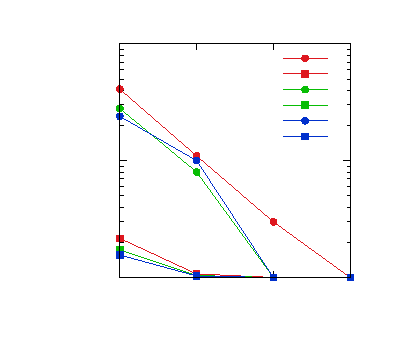
\includegraphics{../plots/encmodules-iwa}}%
    \gplfronttext
  \end{picture}%
\endgroup
 & % GNUPLOT: LaTeX picture with Postscript
\begingroup
\newcommand{\ft}[0]{\footnotesize}\newcommand{\ty}[0]{\tiny}
  \makeatletter
  \providecommand\color[2][]{%
    \GenericError{(gnuplot) \space\space\space\@spaces}{%
      Package color not loaded in conjunction with
      terminal option `colourtext'%
    }{See the gnuplot documentation for explanation.%
    }{Either use 'blacktext' in gnuplot or load the package
      color.sty in LaTeX.}%
    \renewcommand\color[2][]{}%
  }%
  \providecommand\includegraphics[2][]{%
    \GenericError{(gnuplot) \space\space\space\@spaces}{%
      Package graphicx or graphics not loaded%
    }{See the gnuplot documentation for explanation.%
    }{The gnuplot epslatex terminal needs graphicx.sty or graphics.sty.}%
    \renewcommand\includegraphics[2][]{}%
  }%
  \providecommand\rotatebox[2]{#2}%
  \@ifundefined{ifGPcolor}{%
    \newif\ifGPcolor
    \GPcolortrue
  }{}%
  \@ifundefined{ifGPblacktext}{%
    \newif\ifGPblacktext
    \GPblacktextfalse
  }{}%
  % define a \g@addto@macro without @ in the name:
  \let\gplgaddtomacro\g@addto@macro
  % define empty templates for all commands taking text:
  \gdef\gplbacktext{}%
  \gdef\gplfronttext{}%
  \makeatother
  \ifGPblacktext
    % no textcolor at all
    \def\colorrgb#1{}%
    \def\colorgray#1{}%
  \else
    % gray or color?
    \ifGPcolor
      \def\colorrgb#1{\color[rgb]{#1}}%
      \def\colorgray#1{\color[gray]{#1}}%
      \expandafter\def\csname LTw\endcsname{\color{white}}%
      \expandafter\def\csname LTb\endcsname{\color{black}}%
      \expandafter\def\csname LTa\endcsname{\color{black}}%
      \expandafter\def\csname LT0\endcsname{\color[rgb]{1,0,0}}%
      \expandafter\def\csname LT1\endcsname{\color[rgb]{0,1,0}}%
      \expandafter\def\csname LT2\endcsname{\color[rgb]{0,0,1}}%
      \expandafter\def\csname LT3\endcsname{\color[rgb]{1,0,1}}%
      \expandafter\def\csname LT4\endcsname{\color[rgb]{0,1,1}}%
      \expandafter\def\csname LT5\endcsname{\color[rgb]{1,1,0}}%
      \expandafter\def\csname LT6\endcsname{\color[rgb]{0,0,0}}%
      \expandafter\def\csname LT7\endcsname{\color[rgb]{1,0.3,0}}%
      \expandafter\def\csname LT8\endcsname{\color[rgb]{0.5,0.5,0.5}}%
    \else
      % gray
      \def\colorrgb#1{\color{black}}%
      \def\colorgray#1{\color[gray]{#1}}%
      \expandafter\def\csname LTw\endcsname{\color{white}}%
      \expandafter\def\csname LTb\endcsname{\color{black}}%
      \expandafter\def\csname LTa\endcsname{\color{black}}%
      \expandafter\def\csname LT0\endcsname{\color{black}}%
      \expandafter\def\csname LT1\endcsname{\color{black}}%
      \expandafter\def\csname LT2\endcsname{\color{black}}%
      \expandafter\def\csname LT3\endcsname{\color{black}}%
      \expandafter\def\csname LT4\endcsname{\color{black}}%
      \expandafter\def\csname LT5\endcsname{\color{black}}%
      \expandafter\def\csname LT6\endcsname{\color{black}}%
      \expandafter\def\csname LT7\endcsname{\color{black}}%
      \expandafter\def\csname LT8\endcsname{\color{black}}%
    \fi
  \fi
    \setlength{\unitlength}{0.0500bp}%
    \ifx\gptboxheight\undefined%
      \newlength{\gptboxheight}%
      \newlength{\gptboxwidth}%
      \newsavebox{\gptboxtext}%
    \fi%
    \setlength{\fboxrule}{0.5pt}%
    \setlength{\fboxsep}{1pt}%
\begin{picture}(4464.00,3168.00)%
    \gplgaddtomacro\gplbacktext{%
      \csname LTb\endcsname%
      \put(858,660){\makebox(0,0)[r]{\strut{}\ft 1}}%
      \put(858,1782){\makebox(0,0)[r]{\strut{}\ft 10}}%
      \put(858,2903){\makebox(0,0)[r]{\strut{}\ft 100}}%
      \put(990,440){\makebox(0,0){\strut{}\ft 1}}%
      \put(1270,440){\makebox(0,0){\strut{}\ft 2}}%
      \put(1549,440){\makebox(0,0){\strut{}\ft 3}}%
      \put(1829,440){\makebox(0,0){\strut{}\ft 4}}%
      \put(2109,440){\makebox(0,0){\strut{}\ft 5}}%
      \put(2389,440){\makebox(0,0){\strut{}\ft 6}}%
      \put(2668,440){\makebox(0,0){\strut{}\ft 7}}%
      \put(2948,440){\makebox(0,0){\strut{}\ft 8}}%
      \put(3228,440){\makebox(0,0){\strut{}\ft 9}}%
      \put(3508,440){\makebox(0,0){\strut{}\ft 10}}%
      \put(3787,440){\makebox(0,0){\strut{}\ft 11}}%
      \put(4067,440){\makebox(0,0){\strut{}\ft 12}}%
    }%
    \gplgaddtomacro\gplfronttext{%
      \csname LTb\endcsname%
      \put(352,1781){\rotatebox{-270}{\makebox(0,0){\strut{}\ft Enqueued time in cycles}}}%
      \put(2528,154){\makebox(0,0){\strut{}\ft No. of authentication modules}}%
      \csname LTb\endcsname%
      \put(3332,2765){\makebox(0,0)[r]{\strut{}\ty IWA-UC max}}%
      \csname LTb\endcsname%
      \put(3332,2615){\makebox(0,0)[r]{\strut{}\ty avg}}%
      \csname LTb\endcsname%
      \put(3332,2465){\makebox(0,0)[r]{\strut{}\ty G2C3 max}}%
      \csname LTb\endcsname%
      \put(3332,2315){\makebox(0,0)[r]{\strut{}\ty avg}}%
      \csname LTb\endcsname%
      \put(3332,2165){\makebox(0,0)[r]{\strut{}\ty G2C4 max}}%
      \csname LTb\endcsname%
      \put(3332,2015){\makebox(0,0)[r]{\strut{}\ty avg}}%
    }%
    \gplbacktext
    \put(0,0){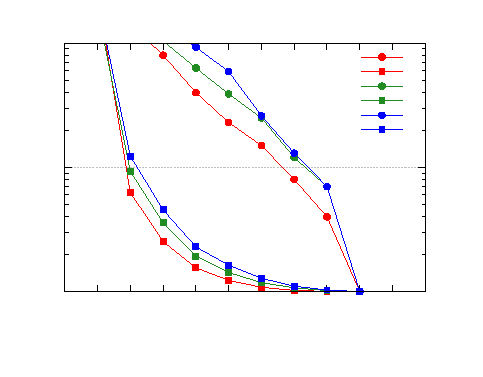
\includegraphics{../plots/authmodules-iwa}}%
    \gplfronttext
  \end{picture}%
\endgroup
 \\
        % GNUPLOT: LaTeX picture with Postscript
\begingroup
\newcommand{\ft}[0]{\footnotesize}\newcommand{\ty}[0]{\tiny}
  \makeatletter
  \providecommand\color[2][]{%
    \GenericError{(gnuplot) \space\space\space\@spaces}{%
      Package color not loaded in conjunction with
      terminal option `colourtext'%
    }{See the gnuplot documentation for explanation.%
    }{Either use 'blacktext' in gnuplot or load the package
      color.sty in LaTeX.}%
    \renewcommand\color[2][]{}%
  }%
  \providecommand\includegraphics[2][]{%
    \GenericError{(gnuplot) \space\space\space\@spaces}{%
      Package graphicx or graphics not loaded%
    }{See the gnuplot documentation for explanation.%
    }{The gnuplot epslatex terminal needs graphicx.sty or graphics.sty.}%
    \renewcommand\includegraphics[2][]{}%
  }%
  \providecommand\rotatebox[2]{#2}%
  \@ifundefined{ifGPcolor}{%
    \newif\ifGPcolor
    \GPcolortrue
  }{}%
  \@ifundefined{ifGPblacktext}{%
    \newif\ifGPblacktext
    \GPblacktextfalse
  }{}%
  % define a \g@addto@macro without @ in the name:
  \let\gplgaddtomacro\g@addto@macro
  % define empty templates for all commands taking text:
  \gdef\gplbacktext{}%
  \gdef\gplfronttext{}%
  \makeatother
  \ifGPblacktext
    % no textcolor at all
    \def\colorrgb#1{}%
    \def\colorgray#1{}%
  \else
    % gray or color?
    \ifGPcolor
      \def\colorrgb#1{\color[rgb]{#1}}%
      \def\colorgray#1{\color[gray]{#1}}%
      \expandafter\def\csname LTw\endcsname{\color{white}}%
      \expandafter\def\csname LTb\endcsname{\color{black}}%
      \expandafter\def\csname LTa\endcsname{\color{black}}%
      \expandafter\def\csname LT0\endcsname{\color[rgb]{1,0,0}}%
      \expandafter\def\csname LT1\endcsname{\color[rgb]{0,1,0}}%
      \expandafter\def\csname LT2\endcsname{\color[rgb]{0,0,1}}%
      \expandafter\def\csname LT3\endcsname{\color[rgb]{1,0,1}}%
      \expandafter\def\csname LT4\endcsname{\color[rgb]{0,1,1}}%
      \expandafter\def\csname LT5\endcsname{\color[rgb]{1,1,0}}%
      \expandafter\def\csname LT6\endcsname{\color[rgb]{0,0,0}}%
      \expandafter\def\csname LT7\endcsname{\color[rgb]{1,0.3,0}}%
      \expandafter\def\csname LT8\endcsname{\color[rgb]{0.5,0.5,0.5}}%
    \else
      % gray
      \def\colorrgb#1{\color{black}}%
      \def\colorgray#1{\color[gray]{#1}}%
      \expandafter\def\csname LTw\endcsname{\color{white}}%
      \expandafter\def\csname LTb\endcsname{\color{black}}%
      \expandafter\def\csname LTa\endcsname{\color{black}}%
      \expandafter\def\csname LT0\endcsname{\color{black}}%
      \expandafter\def\csname LT1\endcsname{\color{black}}%
      \expandafter\def\csname LT2\endcsname{\color{black}}%
      \expandafter\def\csname LT3\endcsname{\color{black}}%
      \expandafter\def\csname LT4\endcsname{\color{black}}%
      \expandafter\def\csname LT5\endcsname{\color{black}}%
      \expandafter\def\csname LT6\endcsname{\color{black}}%
      \expandafter\def\csname LT7\endcsname{\color{black}}%
      \expandafter\def\csname LT8\endcsname{\color{black}}%
    \fi
  \fi
    \setlength{\unitlength}{0.0500bp}%
    \ifx\gptboxheight\undefined%
      \newlength{\gptboxheight}%
      \newlength{\gptboxwidth}%
      \newsavebox{\gptboxtext}%
    \fi%
    \setlength{\fboxrule}{0.5pt}%
    \setlength{\fboxsep}{1pt}%
\begin{picture}(3600.00,3168.00)%
    \gplgaddtomacro\gplbacktext{%
      \csname LTb\endcsname%
      \put(858,660){\makebox(0,0)[r]{\strut{}\ft 1}}%
      \put(858,1782){\makebox(0,0)[r]{\strut{}\ft 10}}%
      \put(858,2903){\makebox(0,0)[r]{\strut{}\ft 100}}%
      \put(990,440){\makebox(0,0){\strut{}\ft 1}}%
      \put(1728,440){\makebox(0,0){\strut{}\ft 2}}%
      \put(2465,440){\makebox(0,0){\strut{}\ft 3}}%
      \put(3203,440){\makebox(0,0){\strut{}\ft 4}}%
    }%
    \gplgaddtomacro\gplfronttext{%
      \csname LTb\endcsname%
      \put(352,1781){\rotatebox{-270}{\makebox(0,0){\strut{}\ft Enqueued time in cycles}}}%
      \put(2096,154){\makebox(0,0){\strut{}\ft No. of encryption modules}}%
      \csname LTb\endcsname%
      \put(2468,2765){\makebox(0,0)[r]{\strut{}\ty FGA-G2C3 max}}%
      \csname LTb\endcsname%
      \put(2468,2615){\makebox(0,0)[r]{\strut{}\ty avg}}%
      \csname LTb\endcsname%
      \put(2468,2465){\makebox(0,0)[r]{\strut{}\ty G2C4 max}}%
      \csname LTb\endcsname%
      \put(2468,2315){\makebox(0,0)[r]{\strut{}\ty avg}}%
    }%
    \gplbacktext
    \put(0,0){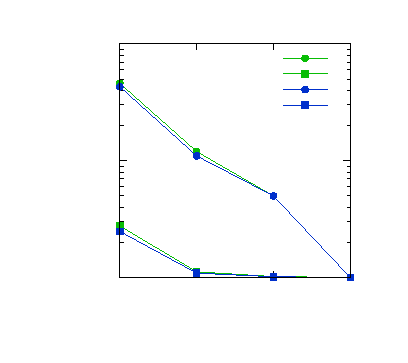
\includegraphics{../plots/encmodules-fga}}%
    \gplfronttext
  \end{picture}%
\endgroup
 & % GNUPLOT: LaTeX picture with Postscript
\begingroup
\newcommand{\ft}[0]{\footnotesize}\newcommand{\ty}[0]{\tiny}
  \makeatletter
  \providecommand\color[2][]{%
    \GenericError{(gnuplot) \space\space\space\@spaces}{%
      Package color not loaded in conjunction with
      terminal option `colourtext'%
    }{See the gnuplot documentation for explanation.%
    }{Either use 'blacktext' in gnuplot or load the package
      color.sty in LaTeX.}%
    \renewcommand\color[2][]{}%
  }%
  \providecommand\includegraphics[2][]{%
    \GenericError{(gnuplot) \space\space\space\@spaces}{%
      Package graphicx or graphics not loaded%
    }{See the gnuplot documentation for explanation.%
    }{The gnuplot epslatex terminal needs graphicx.sty or graphics.sty.}%
    \renewcommand\includegraphics[2][]{}%
  }%
  \providecommand\rotatebox[2]{#2}%
  \@ifundefined{ifGPcolor}{%
    \newif\ifGPcolor
    \GPcolortrue
  }{}%
  \@ifundefined{ifGPblacktext}{%
    \newif\ifGPblacktext
    \GPblacktextfalse
  }{}%
  % define a \g@addto@macro without @ in the name:
  \let\gplgaddtomacro\g@addto@macro
  % define empty templates for all commands taking text:
  \gdef\gplbacktext{}%
  \gdef\gplfronttext{}%
  \makeatother
  \ifGPblacktext
    % no textcolor at all
    \def\colorrgb#1{}%
    \def\colorgray#1{}%
  \else
    % gray or color?
    \ifGPcolor
      \def\colorrgb#1{\color[rgb]{#1}}%
      \def\colorgray#1{\color[gray]{#1}}%
      \expandafter\def\csname LTw\endcsname{\color{white}}%
      \expandafter\def\csname LTb\endcsname{\color{black}}%
      \expandafter\def\csname LTa\endcsname{\color{black}}%
      \expandafter\def\csname LT0\endcsname{\color[rgb]{1,0,0}}%
      \expandafter\def\csname LT1\endcsname{\color[rgb]{0,1,0}}%
      \expandafter\def\csname LT2\endcsname{\color[rgb]{0,0,1}}%
      \expandafter\def\csname LT3\endcsname{\color[rgb]{1,0,1}}%
      \expandafter\def\csname LT4\endcsname{\color[rgb]{0,1,1}}%
      \expandafter\def\csname LT5\endcsname{\color[rgb]{1,1,0}}%
      \expandafter\def\csname LT6\endcsname{\color[rgb]{0,0,0}}%
      \expandafter\def\csname LT7\endcsname{\color[rgb]{1,0.3,0}}%
      \expandafter\def\csname LT8\endcsname{\color[rgb]{0.5,0.5,0.5}}%
    \else
      % gray
      \def\colorrgb#1{\color{black}}%
      \def\colorgray#1{\color[gray]{#1}}%
      \expandafter\def\csname LTw\endcsname{\color{white}}%
      \expandafter\def\csname LTb\endcsname{\color{black}}%
      \expandafter\def\csname LTa\endcsname{\color{black}}%
      \expandafter\def\csname LT0\endcsname{\color{black}}%
      \expandafter\def\csname LT1\endcsname{\color{black}}%
      \expandafter\def\csname LT2\endcsname{\color{black}}%
      \expandafter\def\csname LT3\endcsname{\color{black}}%
      \expandafter\def\csname LT4\endcsname{\color{black}}%
      \expandafter\def\csname LT5\endcsname{\color{black}}%
      \expandafter\def\csname LT6\endcsname{\color{black}}%
      \expandafter\def\csname LT7\endcsname{\color{black}}%
      \expandafter\def\csname LT8\endcsname{\color{black}}%
    \fi
  \fi
    \setlength{\unitlength}{0.0500bp}%
    \ifx\gptboxheight\undefined%
      \newlength{\gptboxheight}%
      \newlength{\gptboxwidth}%
      \newsavebox{\gptboxtext}%
    \fi%
    \setlength{\fboxrule}{0.5pt}%
    \setlength{\fboxsep}{1pt}%
\begin{picture}(4320.00,3310.00)%
    \gplgaddtomacro\gplbacktext{%
      \csname LTb\endcsname%
      \put(330,660){\makebox(0,0)[r]{\strut{}\ft 1}}%
      \csname LTb\endcsname%
      \put(330,1853){\makebox(0,0)[r]{\strut{}\ft 10}}%
      \csname LTb\endcsname%
      \put(330,3045){\makebox(0,0)[r]{\strut{}\ft 100}}%
      \put(462,440){\makebox(0,0){\strut{}\ft 1}}%
      \put(777,440){\makebox(0,0){\strut{}\ft 2}}%
      \put(1091,440){\makebox(0,0){\strut{}\ft 3}}%
      \put(1406,440){\makebox(0,0){\strut{}\ft 4}}%
      \put(1721,440){\makebox(0,0){\strut{}\ft 5}}%
      \put(2035,440){\makebox(0,0){\strut{}\ft 6}}%
      \put(2350,440){\makebox(0,0){\strut{}\ft 7}}%
      \put(2664,440){\makebox(0,0){\strut{}\ft 8}}%
      \put(2979,440){\makebox(0,0){\strut{}\ft 9}}%
      \put(3294,440){\makebox(0,0){\strut{}\ft 10}}%
      \put(3608,440){\makebox(0,0){\strut{}\ft 11}}%
      \put(3923,440){\makebox(0,0){\strut{}\ft 12}}%
    }%
    \gplgaddtomacro\gplfronttext{%
      \csname LTb\endcsname%
      \put(-137,1852){\rotatebox{-270}{\makebox(0,0){\strut{}\ft Enqueued time in cycles}}}%
      \put(2192,154){\makebox(0,0){\strut{}\ft No. of authentication modules}}%
      \csname LTb\endcsname%
      \put(3224,2912){\makebox(0,0)[r]{\strut{}\ty FGA-G2C3 max}}%
      \csname LTb\endcsname%
      \put(3224,2772){\makebox(0,0)[r]{\strut{}\ty avg}}%
      \csname LTb\endcsname%
      \put(3224,2632){\makebox(0,0)[r]{\strut{}\ty G2C4 max}}%
      \csname LTb\endcsname%
      \put(3224,2492){\makebox(0,0)[r]{\strut{}\ty avg}}%
    }%
    \gplbacktext
    \put(0,0){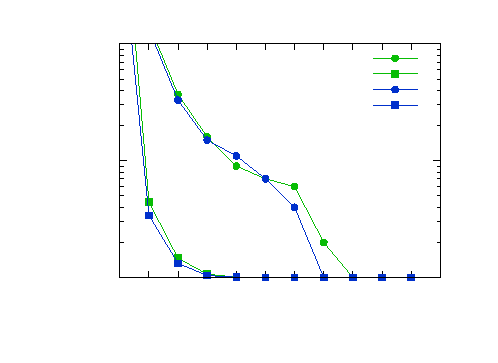
\includegraphics{../plots/authmodules-fga}}%
    \gplfronttext
  \end{picture}%
\endgroup

    \end{tabular}
    \caption[Results for number of crypto modules experiment]{Results for the experiment to determine the number of required crypto modules. The
    number of encryption modules (left column) and authentication modules (right column) is shown in relation to the maximum and average wait times of
    enqueued flits. Each row represents one protocol variant.}
    \label{fig:resultscryptomodules}
\end{figure}

Figure \vref{fig:resultscryptomodules} presents the results of the experiment. For each protocol variant and all viable numbers of encryption and
authentication modules, the maximum and average wait times of flits are depicted. The criterion for having enough modules is that the maximum wait
time should not exceed 10 cycles, while the average should be very close to the minimum of a single cycle. Thus, three encryption and nine
authentication modules are chosen for all subsequent experiments\footnote{This also means that the sizes of the queues in front of the crypto modules
(cf. Figure \ref{fig:omnetni}) do not need to exceed around 10 flits.}.

\subsection{Port Queue Sizes}\label{subsec:portqueuesizes}
The final hyperparameter that is determined is the size of the routers' port queues. This value potentially impacts the transmission delays for
oblivious strategies and has an influence on the routing decisions for adaptive strategies. However, as explained in Section \ref{sec:configurations},
the queue limit is only determined and enforced for \gls{dor} due to the susceptibility of the other strategies to deadlocks. For the adaptive
ones, the determined value is used as a congestion threshold instead of a size limit.

Once again, small queues are preferable with regard to the occupied chip area of the routers, but larger queues are advantageous to achieve lower
transmission latencies. To prevent flits from being discarded due to oversaturation of the network, the local queues of the routers are always
assumed to be unlimited in size. Since \gls{dor} delays flits that are to be routed through a congested link, the flits will accumulate there if the
port queue sizes are too restrictive. Thus, in the experiment, the maximum and average lengths of both the port queues and the local queues are
investigated for varying size limits of the former.

\begin{table}
    \centering
    \begin{tabulary}{\textwidth}{C|C|C|C|C|C|C|C|C|C}
        \pProtVar{} & \pNCMode{} & \pEncMods{} & \pAuthMods{} & \pRQSize{} & \pARQLimit{} & \pARQTimeout{} & \pRStrat{} & \pAttackerSet{} & \pAttackProb{} \\\hline
        \gls{ida} & varying & 3 & 9 & varying & 1 & 12 & \gls{dor} & 1 & 0.2 \\
    \end{tabulary}
    \caption[Input parameters for router queue sizes experiment]{long}
    \label{tab:setupqueuesizes}
\end{table}

The input parameters for the simulator are given in Table \vref{tab:setupqueuesizes}. As the results should be mostly independent of the protocol
variant due to using the same base network injection rates for all of them, \gls{ida} is used as a reference. For the number of crypto modules and the
\gls{arq} timeout, the results of the previous experiments are employed. Attackers are once again present as they may have a considerable impact on
the network load.

\begin{figure}
    \centering
    \begin{tabular}{ll}
        % GNUPLOT: LaTeX picture with Postscript
\begingroup
\newcommand{\ft}[0]{\footnotesize}\newcommand{\ty}[0]{\tiny}
  \makeatletter
  \providecommand\color[2][]{%
    \GenericError{(gnuplot) \space\space\space\@spaces}{%
      Package color not loaded in conjunction with
      terminal option `colourtext'%
    }{See the gnuplot documentation for explanation.%
    }{Either use 'blacktext' in gnuplot or load the package
      color.sty in LaTeX.}%
    \renewcommand\color[2][]{}%
  }%
  \providecommand\includegraphics[2][]{%
    \GenericError{(gnuplot) \space\space\space\@spaces}{%
      Package graphicx or graphics not loaded%
    }{See the gnuplot documentation for explanation.%
    }{The gnuplot epslatex terminal needs graphicx.sty or graphics.sty.}%
    \renewcommand\includegraphics[2][]{}%
  }%
  \providecommand\rotatebox[2]{#2}%
  \@ifundefined{ifGPcolor}{%
    \newif\ifGPcolor
    \GPcolortrue
  }{}%
  \@ifundefined{ifGPblacktext}{%
    \newif\ifGPblacktext
    \GPblacktextfalse
  }{}%
  % define a \g@addto@macro without @ in the name:
  \let\gplgaddtomacro\g@addto@macro
  % define empty templates for all commands taking text:
  \gdef\gplbacktext{}%
  \gdef\gplfronttext{}%
  \makeatother
  \ifGPblacktext
    % no textcolor at all
    \def\colorrgb#1{}%
    \def\colorgray#1{}%
  \else
    % gray or color?
    \ifGPcolor
      \def\colorrgb#1{\color[rgb]{#1}}%
      \def\colorgray#1{\color[gray]{#1}}%
      \expandafter\def\csname LTw\endcsname{\color{white}}%
      \expandafter\def\csname LTb\endcsname{\color{black}}%
      \expandafter\def\csname LTa\endcsname{\color{black}}%
      \expandafter\def\csname LT0\endcsname{\color[rgb]{1,0,0}}%
      \expandafter\def\csname LT1\endcsname{\color[rgb]{0,1,0}}%
      \expandafter\def\csname LT2\endcsname{\color[rgb]{0,0,1}}%
      \expandafter\def\csname LT3\endcsname{\color[rgb]{1,0,1}}%
      \expandafter\def\csname LT4\endcsname{\color[rgb]{0,1,1}}%
      \expandafter\def\csname LT5\endcsname{\color[rgb]{1,1,0}}%
      \expandafter\def\csname LT6\endcsname{\color[rgb]{0,0,0}}%
      \expandafter\def\csname LT7\endcsname{\color[rgb]{1,0.3,0}}%
      \expandafter\def\csname LT8\endcsname{\color[rgb]{0.5,0.5,0.5}}%
    \else
      % gray
      \def\colorrgb#1{\color{black}}%
      \def\colorgray#1{\color[gray]{#1}}%
      \expandafter\def\csname LTw\endcsname{\color{white}}%
      \expandafter\def\csname LTb\endcsname{\color{black}}%
      \expandafter\def\csname LTa\endcsname{\color{black}}%
      \expandafter\def\csname LT0\endcsname{\color{black}}%
      \expandafter\def\csname LT1\endcsname{\color{black}}%
      \expandafter\def\csname LT2\endcsname{\color{black}}%
      \expandafter\def\csname LT3\endcsname{\color{black}}%
      \expandafter\def\csname LT4\endcsname{\color{black}}%
      \expandafter\def\csname LT5\endcsname{\color{black}}%
      \expandafter\def\csname LT6\endcsname{\color{black}}%
      \expandafter\def\csname LT7\endcsname{\color{black}}%
      \expandafter\def\csname LT8\endcsname{\color{black}}%
    \fi
  \fi
    \setlength{\unitlength}{0.0500bp}%
    \ifx\gptboxheight\undefined%
      \newlength{\gptboxheight}%
      \newlength{\gptboxwidth}%
      \newsavebox{\gptboxtext}%
    \fi%
    \setlength{\fboxrule}{0.5pt}%
    \setlength{\fboxsep}{1pt}%
\begin{picture}(4030.00,3600.00)%
    \gplgaddtomacro\gplbacktext{%
      \csname LTb\endcsname%
      \put(990,660){\makebox(0,0)[r]{\strut{}\ft 0.1}}%
      \put(990,1216){\makebox(0,0)[r]{\strut{}\ft 1}}%
      \put(990,1773){\makebox(0,0)[r]{\strut{}\ft 10}}%
      \put(990,2329){\makebox(0,0)[r]{\strut{}\ft 100}}%
      \put(990,2885){\makebox(0,0)[r]{\strut{}\ft 1000}}%
      \put(3633,440){\makebox(0,0){\strut{}$\infty$}}%
      \put(1122,440){\makebox(0,0){\strut{}\ft 1}}%
      \put(1373,440){\makebox(0,0){\strut{}\ft 2}}%
      \put(1624,440){\makebox(0,0){\strut{}\ft 3}}%
      \put(1875,440){\makebox(0,0){\strut{}\ft 4}}%
      \put(2126,440){\makebox(0,0){\strut{}\ft 5}}%
      \put(2378,440){\makebox(0,0){\strut{}\ft 6}}%
      \put(2629,440){\makebox(0,0){\strut{}\ft 7}}%
      \put(2880,440){\makebox(0,0){\strut{}\ft 8}}%
      \put(3131,440){\makebox(0,0){\strut{}\ft 9}}%
      \put(3382,440){\makebox(0,0){\strut{}\ft 10}}%
    }%
    \gplgaddtomacro\gplfronttext{%
      \csname LTb\endcsname%
      \put(352,1772){\rotatebox{-270}{\makebox(0,0){\strut{}\ft Port queue lengths in flits}}}%
      \put(2377,154){\makebox(0,0){\strut{}\ft Maximum port queue size}}%
      \csname LTb\endcsname%
      \put(1774,3462){\makebox(0,0)[r]{\strut{}\ty IDA-UC max}}%
      \csname LTb\endcsname%
      \put(1774,3312){\makebox(0,0)[r]{\strut{}\ty G2C3 max}}%
      \csname LTb\endcsname%
      \put(1774,3162){\makebox(0,0)[r]{\strut{}\ty G2C4 max}}%
      \csname LTb\endcsname%
      \put(3457,3462){\makebox(0,0)[r]{\strut{}\ty avg}}%
      \csname LTb\endcsname%
      \put(3457,3312){\makebox(0,0)[r]{\strut{}\ty avg}}%
      \csname LTb\endcsname%
      \put(3457,3162){\makebox(0,0)[r]{\strut{}\ty avg}}%
    }%
    \gplbacktext
    \put(0,0){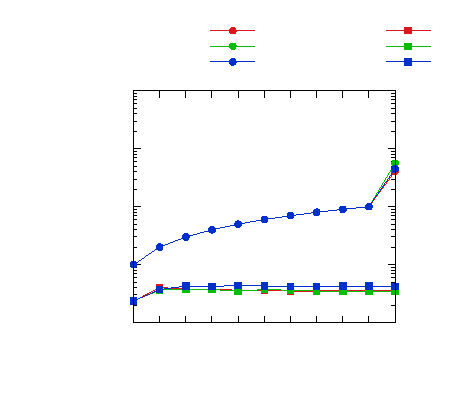
\includegraphics{../plots/queuelengths-ports}}%
    \gplfronttext
  \end{picture}%
\endgroup
 & % GNUPLOT: LaTeX picture with Postscript
\begingroup
\newcommand{\ft}[0]{\footnotesize}\newcommand{\ty}[0]{\tiny}
  \makeatletter
  \providecommand\color[2][]{%
    \GenericError{(gnuplot) \space\space\space\@spaces}{%
      Package color not loaded in conjunction with
      terminal option `colourtext'%
    }{See the gnuplot documentation for explanation.%
    }{Either use 'blacktext' in gnuplot or load the package
      color.sty in LaTeX.}%
    \renewcommand\color[2][]{}%
  }%
  \providecommand\includegraphics[2][]{%
    \GenericError{(gnuplot) \space\space\space\@spaces}{%
      Package graphicx or graphics not loaded%
    }{See the gnuplot documentation for explanation.%
    }{The gnuplot epslatex terminal needs graphicx.sty or graphics.sty.}%
    \renewcommand\includegraphics[2][]{}%
  }%
  \providecommand\rotatebox[2]{#2}%
  \@ifundefined{ifGPcolor}{%
    \newif\ifGPcolor
    \GPcolortrue
  }{}%
  \@ifundefined{ifGPblacktext}{%
    \newif\ifGPblacktext
    \GPblacktextfalse
  }{}%
  % define a \g@addto@macro without @ in the name:
  \let\gplgaddtomacro\g@addto@macro
  % define empty templates for all commands taking text:
  \gdef\gplbacktext{}%
  \gdef\gplfronttext{}%
  \makeatother
  \ifGPblacktext
    % no textcolor at all
    \def\colorrgb#1{}%
    \def\colorgray#1{}%
  \else
    % gray or color?
    \ifGPcolor
      \def\colorrgb#1{\color[rgb]{#1}}%
      \def\colorgray#1{\color[gray]{#1}}%
      \expandafter\def\csname LTw\endcsname{\color{white}}%
      \expandafter\def\csname LTb\endcsname{\color{black}}%
      \expandafter\def\csname LTa\endcsname{\color{black}}%
      \expandafter\def\csname LT0\endcsname{\color[rgb]{1,0,0}}%
      \expandafter\def\csname LT1\endcsname{\color[rgb]{0,1,0}}%
      \expandafter\def\csname LT2\endcsname{\color[rgb]{0,0,1}}%
      \expandafter\def\csname LT3\endcsname{\color[rgb]{1,0,1}}%
      \expandafter\def\csname LT4\endcsname{\color[rgb]{0,1,1}}%
      \expandafter\def\csname LT5\endcsname{\color[rgb]{1,1,0}}%
      \expandafter\def\csname LT6\endcsname{\color[rgb]{0,0,0}}%
      \expandafter\def\csname LT7\endcsname{\color[rgb]{1,0.3,0}}%
      \expandafter\def\csname LT8\endcsname{\color[rgb]{0.5,0.5,0.5}}%
    \else
      % gray
      \def\colorrgb#1{\color{black}}%
      \def\colorgray#1{\color[gray]{#1}}%
      \expandafter\def\csname LTw\endcsname{\color{white}}%
      \expandafter\def\csname LTb\endcsname{\color{black}}%
      \expandafter\def\csname LTa\endcsname{\color{black}}%
      \expandafter\def\csname LT0\endcsname{\color{black}}%
      \expandafter\def\csname LT1\endcsname{\color{black}}%
      \expandafter\def\csname LT2\endcsname{\color{black}}%
      \expandafter\def\csname LT3\endcsname{\color{black}}%
      \expandafter\def\csname LT4\endcsname{\color{black}}%
      \expandafter\def\csname LT5\endcsname{\color{black}}%
      \expandafter\def\csname LT6\endcsname{\color{black}}%
      \expandafter\def\csname LT7\endcsname{\color{black}}%
      \expandafter\def\csname LT8\endcsname{\color{black}}%
    \fi
  \fi
    \setlength{\unitlength}{0.0500bp}%
    \ifx\gptboxheight\undefined%
      \newlength{\gptboxheight}%
      \newlength{\gptboxwidth}%
      \newsavebox{\gptboxtext}%
    \fi%
    \setlength{\fboxrule}{0.5pt}%
    \setlength{\fboxsep}{1pt}%
\begin{picture}(3888.00,3600.00)%
    \gplgaddtomacro\gplbacktext{%
      \csname LTb\endcsname%
      \put(369,638){\makebox(0,0)[r]{\strut{}\ft 0.1}}%
      \csname LTb\endcsname%
      \put(369,1207){\makebox(0,0)[r]{\strut{}\ft 1}}%
      \csname LTb\endcsname%
      \put(369,1777){\makebox(0,0)[r]{\strut{}\ft 10}}%
      \csname LTb\endcsname%
      \put(369,2346){\makebox(0,0)[r]{\strut{}\ft 100}}%
      \csname LTb\endcsname%
      \put(369,2915){\makebox(0,0)[r]{\strut{}\ft 1000}}%
      \put(3491,418){\makebox(0,0){\strut{}$\infty$}}%
      \put(501,418){\makebox(0,0){\strut{}\ft 1}}%
      \put(800,418){\makebox(0,0){\strut{}\ft 2}}%
      \put(1099,418){\makebox(0,0){\strut{}\ft 3}}%
      \put(1398,418){\makebox(0,0){\strut{}\ft 4}}%
      \put(1697,418){\makebox(0,0){\strut{}\ft 5}}%
      \put(1996,418){\makebox(0,0){\strut{}\ft 6}}%
      \put(2295,418){\makebox(0,0){\strut{}\ft 7}}%
      \put(2594,418){\makebox(0,0){\strut{}\ft 8}}%
      \put(2893,418){\makebox(0,0){\strut{}\ft 9}}%
      \put(3192,418){\makebox(0,0){\strut{}\ft 10}}%
    }%
    \gplgaddtomacro\gplfronttext{%
      \csname LTb\endcsname%
      \put(-203,1776){\rotatebox{-270}{\makebox(0,0){\strut{}\ft Local queue lengths in flits}}}%
      \put(1996,154){\makebox(0,0){\strut{}\ft Maximum port queue size}}%
      \csname LTb\endcsname%
      \put(1429,3467){\makebox(0,0)[r]{\strut{}\ty IDA-UC max}}%
      \csname LTb\endcsname%
      \put(1429,3327){\makebox(0,0)[r]{\strut{}\ty G2C3 max}}%
      \csname LTb\endcsname%
      \put(1429,3187){\makebox(0,0)[r]{\strut{}\ty G2C4 max}}%
      \csname LTb\endcsname%
      \put(2500,3467){\makebox(0,0)[r]{\strut{}\ty avg}}%
      \csname LTb\endcsname%
      \put(2500,3327){\makebox(0,0)[r]{\strut{}\ty avg}}%
      \csname LTb\endcsname%
      \put(2500,3187){\makebox(0,0)[r]{\strut{}\ty avg}}%
    }%
    \gplbacktext
    \put(0,0){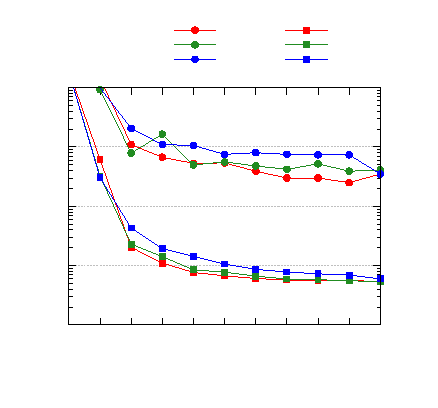
\includegraphics{../plots/queuelengths-local}}%
    \gplfronttext
  \end{picture}%
\endgroup

    \end{tabular}
    \caption[Results for router queue lengths experiment]{long}
    \label{fig:resultsqueuelengths}
\end{figure}

The results are shown in Figure \vref{fig:resultsqueuelengths}. The queue lengths were examined for size restrictions ranging from one to ten flits,
as well as unlimited sizes for comparison. Unsurprisingly, the maximum length of the port queues matches the imposed limit (except for the unlimited
case). Their average length stays relatively constant at approximately 0.4 flits. The more interesting results involve the local queues: with small
size limits on the port queues, flits accumulate there faster than the network can handle them and both maximum and average lengths escalate quickly.
A size limit of six flits was chosen for multiple reasons. First, the average length of the local queues is around one flit, which indicates that even
sporadic accumulations (the highest being 75 flits for G2C4) are dispelled relatively quickly. Second, a higher limit only marginally improves both
average and maximum local queue lengths and is thus not considered worth the additional required chip area.

\section{Performance Comparisons}\label{sec:perfcompeval}
After the preliminary experiments to determine the hyperparameters for the simulations were finished, the main performance evaluations of the protocol
variants and routing strategies are tackled. In the next section, various criteria are established and explained that indicate the performance aspects
of a given configuration. Then, the protocol variants are compared under these criteria for varying attack probabilities of the malicious routers.
Afterwards, the most promising variant is evaluated for each of the presented routing strategies to examine their effects on the performance. Finally,
the consequences of increasing the \gls{arq} limit to 2 are investigated.

\subsection{Criteria}
To facilitate comparisons of the obtained results with previous research at the Chair of Privacy and Data Security of the TU Dresden, the metrics of
\citeauthor{moriam18activeattackers} \cite{moriam18activeattackers} are all adopted for the evaluation here. Those are the acceptance rate, the
information rate, and the residual error probability. As an additional metric, the average end-to-end latency of source flits is employed. The following list elaborates on the
details of these metrics:
\begin{itemize}
    \item \textbf{Acceptance rate.} The base network injection rate specifies the number of flits that are injected into the network per clock cycle
        per node. However, it excludes \glspl{arq} and retransmissions (cf. Section \ref{sec:environmenteval}), whose number rises with increasing
        attack probabilities. By including them, the total network injection rate is obtained, which is called acceptance rate here. It provides an
        indicator for both the frequency of \glspl{arq} and retransmissions as well as the network load.
    \item \textbf{Information rate.} The information rate is the quotient of the amount of created source flits and the total number of flits injected
        into the network. Thus, it illustrates the overhead of authentication, network coding, \glspl{arq}, and retransmissions that the protocol
        imposes for transmitting information from one processing element to another.
    \item \textbf{Residual error probability.} This represents the portion of source flits that were not transmitted successfully to their destination
        processing elements despite exhausting the allowed number of \glspl{arq}. Thus, it serves as a crucial indicator of the reliability and
        resilience that the protocol aims to add to the communications.
    \item \textbf{Average end-to-end latency.} As introduced in Section \ref{sec:networkonchipfun} and mentioned numerous times throughout this
        thesis, low transmission latencies are an essential performance criterion for \glspl{noc}. The average end-to-end latency captures the mean
        transmission time of source flits from their generation at the sending processing elements to their arrival at the receiving ones in clock
        cycles.
\end{itemize}

\subsection{Protocol Variants}
All protocol variants defined in Section \ref{sec:theprotocol} are compared with respect to the performance criteria outlined above. This experiment
aims to identify the most promising one of them. The input parameters of the simulator were chosen according to the results of the preliminary
experiments from Section \ref{sec:hyperparamseval}. The \gls{arq} limit of 1 and the \gls{dor} routing strategy are employed as baselines for the
comparisons once more. The full list of input parameters is given in Table \vref{tab:setupprotvarexperiment}.

\begin{table}
    \centering
    \begin{tabulary}{\textwidth}{C|C|C|C|C|C|C|C|C|C}
        \pProtVar{} & \pNCMode{} & \pEncMods{} & \pAuthMods{} & \pRQSize{} & \pARQLimit{} & \pARQTimeout{} & \pRStrat{} & \pAttackerSet{} & \pAttackProb{} \\\hline
        varying & varying & 3 & 9 & 6 & 1 & 12 & \gls{dor} & all & varying \\
    \end{tabulary}
    \caption[Input parameters for protocol variant experiment]{long}
    \label{tab:setupprotvarexperiment}
\end{table}

The results are presented in Figure \vref{fig:resultsprotvarexperiment}. The four criteria -- acceptance rate, information rate, residual error
probability, and average end-to-end latency -- were investigated for various attack probabilities ranging from 0 to 0.5 to illustrate both the impact
of attackers on the communications and the capability of the different protocol variants to mitigate this impact.

\begin{figure}
    \centering
    \begin{tabular}{ll}
        % GNUPLOT: LaTeX picture with Postscript
\begingroup
\newcommand{\ft}[0]{\footnotesize}\newcommand{\ty}[0]{\tiny}
  \makeatletter
  \providecommand\color[2][]{%
    \GenericError{(gnuplot) \space\space\space\@spaces}{%
      Package color not loaded in conjunction with
      terminal option `colourtext'%
    }{See the gnuplot documentation for explanation.%
    }{Either use 'blacktext' in gnuplot or load the package
      color.sty in LaTeX.}%
    \renewcommand\color[2][]{}%
  }%
  \providecommand\includegraphics[2][]{%
    \GenericError{(gnuplot) \space\space\space\@spaces}{%
      Package graphicx or graphics not loaded%
    }{See the gnuplot documentation for explanation.%
    }{The gnuplot epslatex terminal needs graphicx.sty or graphics.sty.}%
    \renewcommand\includegraphics[2][]{}%
  }%
  \providecommand\rotatebox[2]{#2}%
  \@ifundefined{ifGPcolor}{%
    \newif\ifGPcolor
    \GPcolortrue
  }{}%
  \@ifundefined{ifGPblacktext}{%
    \newif\ifGPblacktext
    \GPblacktextfalse
  }{}%
  % define a \g@addto@macro without @ in the name:
  \let\gplgaddtomacro\g@addto@macro
  % define empty templates for all commands taking text:
  \gdef\gplbacktext{}%
  \gdef\gplfronttext{}%
  \makeatother
  \ifGPblacktext
    % no textcolor at all
    \def\colorrgb#1{}%
    \def\colorgray#1{}%
  \else
    % gray or color?
    \ifGPcolor
      \def\colorrgb#1{\color[rgb]{#1}}%
      \def\colorgray#1{\color[gray]{#1}}%
      \expandafter\def\csname LTw\endcsname{\color{white}}%
      \expandafter\def\csname LTb\endcsname{\color{black}}%
      \expandafter\def\csname LTa\endcsname{\color{black}}%
      \expandafter\def\csname LT0\endcsname{\color[rgb]{1,0,0}}%
      \expandafter\def\csname LT1\endcsname{\color[rgb]{0,1,0}}%
      \expandafter\def\csname LT2\endcsname{\color[rgb]{0,0,1}}%
      \expandafter\def\csname LT3\endcsname{\color[rgb]{1,0,1}}%
      \expandafter\def\csname LT4\endcsname{\color[rgb]{0,1,1}}%
      \expandafter\def\csname LT5\endcsname{\color[rgb]{1,1,0}}%
      \expandafter\def\csname LT6\endcsname{\color[rgb]{0,0,0}}%
      \expandafter\def\csname LT7\endcsname{\color[rgb]{1,0.3,0}}%
      \expandafter\def\csname LT8\endcsname{\color[rgb]{0.5,0.5,0.5}}%
    \else
      % gray
      \def\colorrgb#1{\color{black}}%
      \def\colorgray#1{\color[gray]{#1}}%
      \expandafter\def\csname LTw\endcsname{\color{white}}%
      \expandafter\def\csname LTb\endcsname{\color{black}}%
      \expandafter\def\csname LTa\endcsname{\color{black}}%
      \expandafter\def\csname LT0\endcsname{\color{black}}%
      \expandafter\def\csname LT1\endcsname{\color{black}}%
      \expandafter\def\csname LT2\endcsname{\color{black}}%
      \expandafter\def\csname LT3\endcsname{\color{black}}%
      \expandafter\def\csname LT4\endcsname{\color{black}}%
      \expandafter\def\csname LT5\endcsname{\color{black}}%
      \expandafter\def\csname LT6\endcsname{\color{black}}%
      \expandafter\def\csname LT7\endcsname{\color{black}}%
      \expandafter\def\csname LT8\endcsname{\color{black}}%
    \fi
  \fi
    \setlength{\unitlength}{0.0500bp}%
    \ifx\gptboxheight\undefined%
      \newlength{\gptboxheight}%
      \newlength{\gptboxwidth}%
      \newsavebox{\gptboxtext}%
    \fi%
    \setlength{\fboxrule}{0.5pt}%
    \setlength{\fboxsep}{1pt}%
\begin{picture}(4030.00,3600.00)%
    \gplgaddtomacro\gplbacktext{%
      \csname LTb\endcsname%
      \put(990,660){\makebox(0,0)[r]{\strut{}\ty 0.2}}%
      \put(990,868){\makebox(0,0)[r]{\strut{}\ty 0.21}}%
      \put(990,1075){\makebox(0,0)[r]{\strut{}\ty 0.22}}%
      \put(990,1283){\makebox(0,0)[r]{\strut{}\ty 0.23}}%
      \put(990,1490){\makebox(0,0)[r]{\strut{}\ty 0.24}}%
      \put(990,1698){\makebox(0,0)[r]{\strut{}\ty 0.25}}%
      \put(990,1905){\makebox(0,0)[r]{\strut{}\ty 0.26}}%
      \put(990,2113){\makebox(0,0)[r]{\strut{}\ty 0.27}}%
      \put(990,2320){\makebox(0,0)[r]{\strut{}\ty 0.28}}%
      \put(990,2528){\makebox(0,0)[r]{\strut{}\ty 0.29}}%
      \put(990,2735){\makebox(0,0)[r]{\strut{}\ty 0.3}}%
      \put(1122,440){\makebox(0,0){\strut{}\ty 0}}%
      \put(2063,440){\makebox(0,0){\strut{}\ty 0.1}}%
      \put(3004,440){\makebox(0,0){\strut{}\ty 0.2}}%
      \put(3192,440){\makebox(0,0){\strut{}}}%
      \put(3380,440){\makebox(0,0){\strut{}}}%
      \put(3568,440){\makebox(0,0){\strut{}\ty 0.5}}%
    }%
    \gplgaddtomacro\gplfronttext{%
      \csname LTb\endcsname%
      \put(352,1697){\rotatebox{-270}{\makebox(0,0){\strut{}\ft Acceptance rate}}}%
      \put(2345,154){\makebox(0,0){\strut{}\ft Attack probabilities}}%
      \csname LTb\endcsname%
      \put(1742,3462){\makebox(0,0)[r]{\strut{}\ty IDA-UC}}%
      \csname LTb\endcsname%
      \put(1742,3312){\makebox(0,0)[r]{\strut{}\ty G2C3}}%
      \csname LTb\endcsname%
      \put(1742,3162){\makebox(0,0)[r]{\strut{}\ty G2C4}}%
      \csname LTb\endcsname%
      \put(1742,3012){\makebox(0,0)[r]{\strut{}\ty IWA-UC}}%
      \csname LTb\endcsname%
      \put(3245,3462){\makebox(0,0)[r]{\strut{}\ty G2C3}}%
      \csname LTb\endcsname%
      \put(3245,3312){\makebox(0,0)[r]{\strut{}\ty G2C4}}%
      \csname LTb\endcsname%
      \put(3245,3162){\makebox(0,0)[r]{\strut{}\ty FGA-G2C3}}%
      \csname LTb\endcsname%
      \put(3245,3012){\makebox(0,0)[r]{\strut{}\ty FGA-G2C4}}%
    }%
    \gplbacktext
    \put(0,0){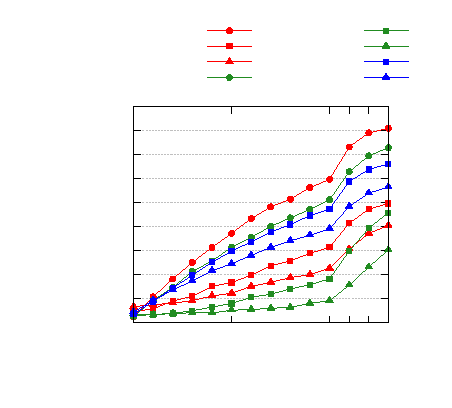
\includegraphics{../plots/main-acceptancerate}}%
    \gplfronttext
  \end{picture}%
\endgroup
 & % GNUPLOT: LaTeX picture with Postscript
\begingroup
\newcommand{\ft}[0]{\footnotesize}\newcommand{\ty}[0]{\tiny}
  \makeatletter
  \providecommand\color[2][]{%
    \GenericError{(gnuplot) \space\space\space\@spaces}{%
      Package color not loaded in conjunction with
      terminal option `colourtext'%
    }{See the gnuplot documentation for explanation.%
    }{Either use 'blacktext' in gnuplot or load the package
      color.sty in LaTeX.}%
    \renewcommand\color[2][]{}%
  }%
  \providecommand\includegraphics[2][]{%
    \GenericError{(gnuplot) \space\space\space\@spaces}{%
      Package graphicx or graphics not loaded%
    }{See the gnuplot documentation for explanation.%
    }{The gnuplot epslatex terminal needs graphicx.sty or graphics.sty.}%
    \renewcommand\includegraphics[2][]{}%
  }%
  \providecommand\rotatebox[2]{#2}%
  \@ifundefined{ifGPcolor}{%
    \newif\ifGPcolor
    \GPcolortrue
  }{}%
  \@ifundefined{ifGPblacktext}{%
    \newif\ifGPblacktext
    \GPblacktextfalse
  }{}%
  % define a \g@addto@macro without @ in the name:
  \let\gplgaddtomacro\g@addto@macro
  % define empty templates for all commands taking text:
  \gdef\gplbacktext{}%
  \gdef\gplfronttext{}%
  \makeatother
  \ifGPblacktext
    % no textcolor at all
    \def\colorrgb#1{}%
    \def\colorgray#1{}%
  \else
    % gray or color?
    \ifGPcolor
      \def\colorrgb#1{\color[rgb]{#1}}%
      \def\colorgray#1{\color[gray]{#1}}%
      \expandafter\def\csname LTw\endcsname{\color{white}}%
      \expandafter\def\csname LTb\endcsname{\color{black}}%
      \expandafter\def\csname LTa\endcsname{\color{black}}%
      \expandafter\def\csname LT0\endcsname{\color[rgb]{1,0,0}}%
      \expandafter\def\csname LT1\endcsname{\color[rgb]{0,1,0}}%
      \expandafter\def\csname LT2\endcsname{\color[rgb]{0,0,1}}%
      \expandafter\def\csname LT3\endcsname{\color[rgb]{1,0,1}}%
      \expandafter\def\csname LT4\endcsname{\color[rgb]{0,1,1}}%
      \expandafter\def\csname LT5\endcsname{\color[rgb]{1,1,0}}%
      \expandafter\def\csname LT6\endcsname{\color[rgb]{0,0,0}}%
      \expandafter\def\csname LT7\endcsname{\color[rgb]{1,0.3,0}}%
      \expandafter\def\csname LT8\endcsname{\color[rgb]{0.5,0.5,0.5}}%
    \else
      % gray
      \def\colorrgb#1{\color{black}}%
      \def\colorgray#1{\color[gray]{#1}}%
      \expandafter\def\csname LTw\endcsname{\color{white}}%
      \expandafter\def\csname LTb\endcsname{\color{black}}%
      \expandafter\def\csname LTa\endcsname{\color{black}}%
      \expandafter\def\csname LT0\endcsname{\color{black}}%
      \expandafter\def\csname LT1\endcsname{\color{black}}%
      \expandafter\def\csname LT2\endcsname{\color{black}}%
      \expandafter\def\csname LT3\endcsname{\color{black}}%
      \expandafter\def\csname LT4\endcsname{\color{black}}%
      \expandafter\def\csname LT5\endcsname{\color{black}}%
      \expandafter\def\csname LT6\endcsname{\color{black}}%
      \expandafter\def\csname LT7\endcsname{\color{black}}%
      \expandafter\def\csname LT8\endcsname{\color{black}}%
    \fi
  \fi
    \setlength{\unitlength}{0.0500bp}%
    \ifx\gptboxheight\undefined%
      \newlength{\gptboxheight}%
      \newlength{\gptboxwidth}%
      \newsavebox{\gptboxtext}%
    \fi%
    \setlength{\fboxrule}{0.5pt}%
    \setlength{\fboxsep}{1pt}%
\begin{picture}(3744.00,4320.00)%
    \gplgaddtomacro\gplbacktext{%
      \csname LTb\endcsname%
      \put(369,638){\makebox(0,0)[r]{\strut{}\ft 0.2}}%
      \csname LTb\endcsname%
      \put(369,1114){\makebox(0,0)[r]{\strut{}\ft 0.25}}%
      \csname LTb\endcsname%
      \put(369,1590){\makebox(0,0)[r]{\strut{}\ft 0.3}}%
      \csname LTb\endcsname%
      \put(369,2067){\makebox(0,0)[r]{\strut{}\ft 0.35}}%
      \csname LTb\endcsname%
      \put(369,2543){\makebox(0,0)[r]{\strut{}\ft 0.4}}%
      \csname LTb\endcsname%
      \put(369,3019){\makebox(0,0)[r]{\strut{}\ft 0.45}}%
      \csname LTb\endcsname%
      \put(369,3495){\makebox(0,0)[r]{\strut{}\ft 0.5}}%
      \put(501,418){\makebox(0,0){\strut{}\ft 0}}%
      \put(1571,418){\makebox(0,0){\strut{}\ft 0.1}}%
      \put(2640,418){\makebox(0,0){\strut{}\ft 0.2}}%
      \put(2854,418){\makebox(0,0){\strut{}}}%
      \put(3068,418){\makebox(0,0){\strut{}}}%
      \put(3282,418){\makebox(0,0){\strut{}\ft 0.5}}%
    }%
    \gplgaddtomacro\gplfronttext{%
      \csname LTb\endcsname%
      \put(-190,2066){\rotatebox{-270}{\makebox(0,0){\strut{}\ft Information rate}}}%
      \put(1891,154){\makebox(0,0){\strut{}\ft Attack probabilities}}%
      \csname LTb\endcsname%
      \put(1324,4187){\makebox(0,0)[r]{\strut{}\ty IDA-UC}}%
      \csname LTb\endcsname%
      \put(1324,4047){\makebox(0,0)[r]{\strut{}\ty G2C3}}%
      \csname LTb\endcsname%
      \put(1324,3907){\makebox(0,0)[r]{\strut{}\ty G2C4}}%
      \csname LTb\endcsname%
      \put(1324,3767){\makebox(0,0)[r]{\strut{}\ty IWA-UC}}%
      \csname LTb\endcsname%
      \put(2731,4187){\makebox(0,0)[r]{\strut{}\ty G2C3}}%
      \csname LTb\endcsname%
      \put(2731,4047){\makebox(0,0)[r]{\strut{}\ty G2C4}}%
      \csname LTb\endcsname%
      \put(2731,3907){\makebox(0,0)[r]{\strut{}\ty FGA-G2C3}}%
      \csname LTb\endcsname%
      \put(2731,3767){\makebox(0,0)[r]{\strut{}\ty G2C4}}%
    }%
    \gplbacktext
    \put(0,0){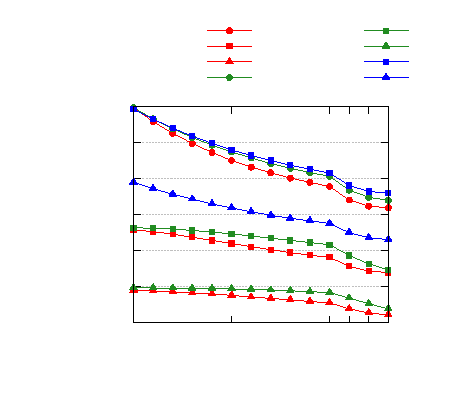
\includegraphics{../plots/main-informationrate}}%
    \gplfronttext
  \end{picture}%
\endgroup
 \\
        % GNUPLOT: LaTeX picture with Postscript
\begingroup
\newcommand{\ft}[0]{\footnotesize}\newcommand{\ty}[0]{\tiny}
  \makeatletter
  \providecommand\color[2][]{%
    \GenericError{(gnuplot) \space\space\space\@spaces}{%
      Package color not loaded in conjunction with
      terminal option `colourtext'%
    }{See the gnuplot documentation for explanation.%
    }{Either use 'blacktext' in gnuplot or load the package
      color.sty in LaTeX.}%
    \renewcommand\color[2][]{}%
  }%
  \providecommand\includegraphics[2][]{%
    \GenericError{(gnuplot) \space\space\space\@spaces}{%
      Package graphicx or graphics not loaded%
    }{See the gnuplot documentation for explanation.%
    }{The gnuplot epslatex terminal needs graphicx.sty or graphics.sty.}%
    \renewcommand\includegraphics[2][]{}%
  }%
  \providecommand\rotatebox[2]{#2}%
  \@ifundefined{ifGPcolor}{%
    \newif\ifGPcolor
    \GPcolortrue
  }{}%
  \@ifundefined{ifGPblacktext}{%
    \newif\ifGPblacktext
    \GPblacktextfalse
  }{}%
  % define a \g@addto@macro without @ in the name:
  \let\gplgaddtomacro\g@addto@macro
  % define empty templates for all commands taking text:
  \gdef\gplbacktext{}%
  \gdef\gplfronttext{}%
  \makeatother
  \ifGPblacktext
    % no textcolor at all
    \def\colorrgb#1{}%
    \def\colorgray#1{}%
  \else
    % gray or color?
    \ifGPcolor
      \def\colorrgb#1{\color[rgb]{#1}}%
      \def\colorgray#1{\color[gray]{#1}}%
      \expandafter\def\csname LTw\endcsname{\color{white}}%
      \expandafter\def\csname LTb\endcsname{\color{black}}%
      \expandafter\def\csname LTa\endcsname{\color{black}}%
      \expandafter\def\csname LT0\endcsname{\color[rgb]{1,0,0}}%
      \expandafter\def\csname LT1\endcsname{\color[rgb]{0,1,0}}%
      \expandafter\def\csname LT2\endcsname{\color[rgb]{0,0,1}}%
      \expandafter\def\csname LT3\endcsname{\color[rgb]{1,0,1}}%
      \expandafter\def\csname LT4\endcsname{\color[rgb]{0,1,1}}%
      \expandafter\def\csname LT5\endcsname{\color[rgb]{1,1,0}}%
      \expandafter\def\csname LT6\endcsname{\color[rgb]{0,0,0}}%
      \expandafter\def\csname LT7\endcsname{\color[rgb]{1,0.3,0}}%
      \expandafter\def\csname LT8\endcsname{\color[rgb]{0.5,0.5,0.5}}%
    \else
      % gray
      \def\colorrgb#1{\color{black}}%
      \def\colorgray#1{\color[gray]{#1}}%
      \expandafter\def\csname LTw\endcsname{\color{white}}%
      \expandafter\def\csname LTb\endcsname{\color{black}}%
      \expandafter\def\csname LTa\endcsname{\color{black}}%
      \expandafter\def\csname LT0\endcsname{\color{black}}%
      \expandafter\def\csname LT1\endcsname{\color{black}}%
      \expandafter\def\csname LT2\endcsname{\color{black}}%
      \expandafter\def\csname LT3\endcsname{\color{black}}%
      \expandafter\def\csname LT4\endcsname{\color{black}}%
      \expandafter\def\csname LT5\endcsname{\color{black}}%
      \expandafter\def\csname LT6\endcsname{\color{black}}%
      \expandafter\def\csname LT7\endcsname{\color{black}}%
      \expandafter\def\csname LT8\endcsname{\color{black}}%
    \fi
  \fi
    \setlength{\unitlength}{0.0500bp}%
    \ifx\gptboxheight\undefined%
      \newlength{\gptboxheight}%
      \newlength{\gptboxwidth}%
      \newsavebox{\gptboxtext}%
    \fi%
    \setlength{\fboxrule}{0.5pt}%
    \setlength{\fboxsep}{1pt}%
\begin{picture}(4030.00,4320.00)%
    \gplgaddtomacro\gplbacktext{%
      \csname LTb\endcsname%
      \put(528,638){\makebox(0,0)[r]{\strut{}\ft 0}}%
      \csname LTb\endcsname%
      \put(528,1157){\makebox(0,0)[r]{\strut{}\ft 0.1}}%
      \csname LTb\endcsname%
      \put(528,1677){\makebox(0,0)[r]{\strut{}\ft 0.2}}%
      \csname LTb\endcsname%
      \put(528,2196){\makebox(0,0)[r]{\strut{}\ft 0.3}}%
      \csname LTb\endcsname%
      \put(528,2716){\makebox(0,0)[r]{\strut{}\ft 0.4}}%
      \csname LTb\endcsname%
      \put(528,3235){\makebox(0,0)[r]{\strut{}\ft 0.5}}%
      \put(660,418){\makebox(0,0){\strut{}\ft 0}}%
      \put(1778,418){\makebox(0,0){\strut{}\ft 0.1}}%
      \put(2897,418){\makebox(0,0){\strut{}\ft 0.2}}%
      \put(3121,418){\makebox(0,0){\strut{}}}%
      \put(3344,418){\makebox(0,0){\strut{}}}%
      \put(3568,418){\makebox(0,0){\strut{}\ft 0.5}}%
    }%
    \gplgaddtomacro\gplfronttext{%
      \csname LTb\endcsname%
      \put(61,2066){\rotatebox{-270}{\makebox(0,0){\strut{}\ft Residual error probability}}}%
      \put(2114,154){\makebox(0,0){\strut{}\ft Attack probabilities}}%
      \csname LTb\endcsname%
      \put(1547,4187){\makebox(0,0)[r]{\strut{}\ty IDA-UC}}%
      \csname LTb\endcsname%
      \put(1547,4047){\makebox(0,0)[r]{\strut{}\ty G2C3}}%
      \csname LTb\endcsname%
      \put(1547,3907){\makebox(0,0)[r]{\strut{}\ty G2C4}}%
      \csname LTb\endcsname%
      \put(1547,3767){\makebox(0,0)[r]{\strut{}\ty IWA-UC}}%
      \csname LTb\endcsname%
      \put(2954,4187){\makebox(0,0)[r]{\strut{}\ty G2C3}}%
      \csname LTb\endcsname%
      \put(2954,4047){\makebox(0,0)[r]{\strut{}\ty G2C4}}%
      \csname LTb\endcsname%
      \put(2954,3907){\makebox(0,0)[r]{\strut{}\ty FGA-G2C3}}%
      \csname LTb\endcsname%
      \put(2954,3767){\makebox(0,0)[r]{\strut{}\ty G2C4}}%
    }%
    \gplbacktext
    \put(0,0){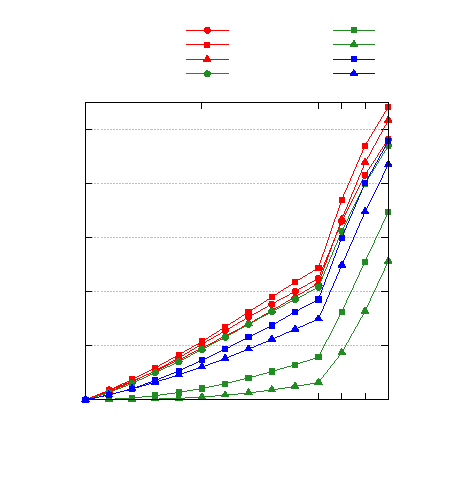
\includegraphics{../plots/main-residualerror}}%
    \gplfronttext
  \end{picture}%
\endgroup
 & % GNUPLOT: LaTeX picture with Postscript
\begingroup
\newcommand{\ft}[0]{\footnotesize}\newcommand{\ty}[0]{\tiny}
  \makeatletter
  \providecommand\color[2][]{%
    \GenericError{(gnuplot) \space\space\space\@spaces}{%
      Package color not loaded in conjunction with
      terminal option `colourtext'%
    }{See the gnuplot documentation for explanation.%
    }{Either use 'blacktext' in gnuplot or load the package
      color.sty in LaTeX.}%
    \renewcommand\color[2][]{}%
  }%
  \providecommand\includegraphics[2][]{%
    \GenericError{(gnuplot) \space\space\space\@spaces}{%
      Package graphicx or graphics not loaded%
    }{See the gnuplot documentation for explanation.%
    }{The gnuplot epslatex terminal needs graphicx.sty or graphics.sty.}%
    \renewcommand\includegraphics[2][]{}%
  }%
  \providecommand\rotatebox[2]{#2}%
  \@ifundefined{ifGPcolor}{%
    \newif\ifGPcolor
    \GPcolortrue
  }{}%
  \@ifundefined{ifGPblacktext}{%
    \newif\ifGPblacktext
    \GPblacktextfalse
  }{}%
  % define a \g@addto@macro without @ in the name:
  \let\gplgaddtomacro\g@addto@macro
  % define empty templates for all commands taking text:
  \gdef\gplbacktext{}%
  \gdef\gplfronttext{}%
  \makeatother
  \ifGPblacktext
    % no textcolor at all
    \def\colorrgb#1{}%
    \def\colorgray#1{}%
  \else
    % gray or color?
    \ifGPcolor
      \def\colorrgb#1{\color[rgb]{#1}}%
      \def\colorgray#1{\color[gray]{#1}}%
      \expandafter\def\csname LTw\endcsname{\color{white}}%
      \expandafter\def\csname LTb\endcsname{\color{black}}%
      \expandafter\def\csname LTa\endcsname{\color{black}}%
      \expandafter\def\csname LT0\endcsname{\color[rgb]{1,0,0}}%
      \expandafter\def\csname LT1\endcsname{\color[rgb]{0,1,0}}%
      \expandafter\def\csname LT2\endcsname{\color[rgb]{0,0,1}}%
      \expandafter\def\csname LT3\endcsname{\color[rgb]{1,0,1}}%
      \expandafter\def\csname LT4\endcsname{\color[rgb]{0,1,1}}%
      \expandafter\def\csname LT5\endcsname{\color[rgb]{1,1,0}}%
      \expandafter\def\csname LT6\endcsname{\color[rgb]{0,0,0}}%
      \expandafter\def\csname LT7\endcsname{\color[rgb]{1,0.3,0}}%
      \expandafter\def\csname LT8\endcsname{\color[rgb]{0.5,0.5,0.5}}%
    \else
      % gray
      \def\colorrgb#1{\color{black}}%
      \def\colorgray#1{\color[gray]{#1}}%
      \expandafter\def\csname LTw\endcsname{\color{white}}%
      \expandafter\def\csname LTb\endcsname{\color{black}}%
      \expandafter\def\csname LTa\endcsname{\color{black}}%
      \expandafter\def\csname LT0\endcsname{\color{black}}%
      \expandafter\def\csname LT1\endcsname{\color{black}}%
      \expandafter\def\csname LT2\endcsname{\color{black}}%
      \expandafter\def\csname LT3\endcsname{\color{black}}%
      \expandafter\def\csname LT4\endcsname{\color{black}}%
      \expandafter\def\csname LT5\endcsname{\color{black}}%
      \expandafter\def\csname LT6\endcsname{\color{black}}%
      \expandafter\def\csname LT7\endcsname{\color{black}}%
      \expandafter\def\csname LT8\endcsname{\color{black}}%
    \fi
  \fi
    \setlength{\unitlength}{0.0500bp}%
    \ifx\gptboxheight\undefined%
      \newlength{\gptboxheight}%
      \newlength{\gptboxwidth}%
      \newsavebox{\gptboxtext}%
    \fi%
    \setlength{\fboxrule}{0.5pt}%
    \setlength{\fboxsep}{1pt}%
\begin{picture}(3744.00,4320.00)%
    \gplgaddtomacro\gplbacktext{%
      \csname LTb\endcsname%
      \put(369,768){\makebox(0,0)[r]{\strut{}\ft 30}}%
      \csname LTb\endcsname%
      \put(369,1417){\makebox(0,0)[r]{\strut{}\ft 35}}%
      \csname LTb\endcsname%
      \put(369,2067){\makebox(0,0)[r]{\strut{}\ft 40}}%
      \csname LTb\endcsname%
      \put(369,2716){\makebox(0,0)[r]{\strut{}\ft 45}}%
      \csname LTb\endcsname%
      \put(369,3365){\makebox(0,0)[r]{\strut{}\ft 50}}%
      \put(501,418){\makebox(0,0){\strut{}\ft 0}}%
      \put(1571,418){\makebox(0,0){\strut{}\ft 0.1}}%
      \put(2640,418){\makebox(0,0){\strut{}\ft 0.2}}%
      \put(2854,418){\makebox(0,0){\strut{}}}%
      \put(3068,418){\makebox(0,0){\strut{}}}%
      \put(3282,418){\makebox(0,0){\strut{}\ft 0.5}}%
    }%
    \gplgaddtomacro\gplfronttext{%
      \csname LTb\endcsname%
      \put(-58,2066){\rotatebox{-270}{\makebox(0,0){\strut{}\ft Avg. end-to-end latency in cycles}}}%
      \put(1891,154){\makebox(0,0){\strut{}\ft Attack probabilities}}%
      \csname LTb\endcsname%
      \put(1324,4187){\makebox(0,0)[r]{\strut{}\ty IDA-UC}}%
      \csname LTb\endcsname%
      \put(1324,4047){\makebox(0,0)[r]{\strut{}\ty G2C3}}%
      \csname LTb\endcsname%
      \put(1324,3907){\makebox(0,0)[r]{\strut{}\ty G2C4}}%
      \csname LTb\endcsname%
      \put(1324,3767){\makebox(0,0)[r]{\strut{}\ty IWA-UC}}%
      \csname LTb\endcsname%
      \put(2731,4187){\makebox(0,0)[r]{\strut{}\ty G2C3}}%
      \csname LTb\endcsname%
      \put(2731,4047){\makebox(0,0)[r]{\strut{}\ty G2C4}}%
      \csname LTb\endcsname%
      \put(2731,3907){\makebox(0,0)[r]{\strut{}\ty FGA-G2C3}}%
      \csname LTb\endcsname%
      \put(2731,3767){\makebox(0,0)[r]{\strut{}\ty G2C4}}%
    }%
    \gplbacktext
    \put(0,0){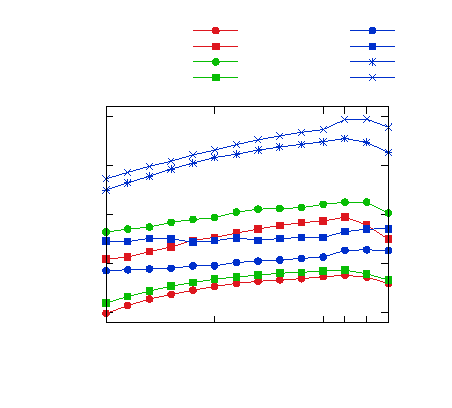
\includegraphics{../plots/main-endtoendlatency}}%
    \gplfronttext
  \end{picture}%
\endgroup

    \end{tabular}
    \caption[Results for protocol variant experiment]{long}
    \label{fig:resultsprotvarexperiment}
\end{figure}

The acceptance rate rises with increasing attack probabilities as more \glspl{arq} and retransmissions become necessary. It starts at slightly
above the base network injection rate of 0.2 even without the presence of malicious routers. This is due to a few sporadic \glspl{arq} that are
triggered by timeouts stemming from temporarily increased network loads; the experiment in Section \ref{subsec:arqtimeouts} already confirmed that
this is possible. With rising attack probabilities, different growth rates can be observed for the protocol variants, indicating that some entail more
\glspl{arq} and retransmissions than others. Unsurprisingly, the uncoded versions are in the lead as they cannot recover from flit loss or
modifications without issuing an \gls{arq}. Following them are the \gls{fga} variants. With only one \gls{mac} for a whole generation, an attack on
the carrying flit always necessitates a retransmission. The lowest acceptance rates are achieved by network coded \gls{ida} and \gls{iwa} as they are
resilient to sporadic attacks and no single modification or loss within a generation forces an \gls{arq}. In general, the G2C4 versions perform better
than G2C3 due to their increased redundancy in the transmitted flits.

The information rate directly reflects the overhead that each protocol variant imposes on the transmissions (cf. Table \ref{tab:creationrates}). Thus,
for no attackers, it is around 0.5 for the uncoded protocols and \gls{fga}-G2C3, as they cause two flits to be injected into the network per source
flit. For \gls{ida} and \gls{iwa} in their G2C4 variants, the overhead is twice as high, resulting in half the information rate. With increasing
attack probabilities, the number of \glspl{arq} are retransmissions rises, which is reflected in declining information rates. In addition, as the
acceptance rate and information rate both indicate the portion of \glspl{arq} and retransmissions of the total traffic, high fluctuations in the
former are accompanied by large variations of the latter.

The residual error probability is the main indicator for the ability of the protocol to mitigate the impact of attackers. Unsurprisingly, a lack of
adversaries results in no residual errors for all variants, but this begins to deviate quickly as the attack probabilities are increased. As expected,
the uncoded versions are both at the worse end of the spectrum. Peculiarly, for \gls{ida}, the network coded versions perform even worse than the
uncoded one, which contrasts with the expectation of their greater resilience. This is likely due to a combination of three properties: first, network
coded \gls{ida} binds two source flits within a single generation, so on average there are only 0.5 \glspl{arq} available per source flit (assuming an
\gls{arq} limit of 1). Second, it comprises the largest transmission units (6 and 8 flits for G2C3 and G2C4, respectively), so the probability of at
least one of these flits being attacked is relatively high. Third, four flits are required to arrive intactly per generation, which is the largest
amount out of all protocol variants. Due to the large transmission units, the necessity of further \glspl{arq} might only be detected when
their limit was already reached, leading to both source flits of the affected generation being lost. This line of thought also explains why network
coded \gls{iwa} performs best: it has the smallest transmission units of all network coded variants, each source flit is comprised within its own
generation, and one \gls{arq} is available for every source flit. \Gls{fga} lying in the middle is explained by the susceptibility of the \gls{mac}
flits: if such a flit is attacked, the complete generation must be retransmitted, as it authenticates both source flits together. Moreover, \gls{fga}
suffers from the same deficit as \gls{ida}: one failing generation entails two lost source flits.

The average end-to-end latency reflects the added expenditure of time required by the protocols to transmit information. Overall, higher attack
probabilities result in increased latencies due to the higher amount of retransmissions. It is important to note that lost source flits, i.e., those
counting towards the residual error probability, are ignored in this statistic as they do not have an end-to-end latency. This also explains the
turnaround at the highest attack probabilities as the retransmissions become increasingly likely to fail. As expected, \gls{fga} has by far the
highest average latencies across all investigated attack probabilities. The reason for this is the duration of the authentication procedure: with 10
cycles, it consumes more time than for \gls{ida} and \gls{iwa} by a large margin. Furthermore, receivers need to obtain enough flits to decode the
generation before the \gls{mac} computation can begin. The uncoded protocol variants have the lowest latencies since no delays are imposed by network
encoding and decoding.

Overall, the network coded versions of \gls{iwa} perform best. While the redundancy entailed by network coding leads to a relatively low information
rate, they provide the most reliable transmissions by a large margin and generate the lowest network load with a competitive average latency. For
these reasons, \gls{iwa} is chosen to be investigated further in the following section.

\subsection{Routing Strategies}
Take: best protocol variant (IWA), use it to find the best routing strategy

\begin{table}
    \centering
    \begin{tabulary}{\textwidth}{C|C|C|C|C|C|C|C|C|C}
        \pProtVar{} & \pNCMode{} & \pEncMods{} & \pAuthMods{} & \pRQSize{} & \pARQLimit{} & \pARQTimeout{} & \pRStrat{} & \pAttackerSet{} & \pAttackProb{} \\\hline
        \gls{iwa} & varying & 3 & 9 & 6 & 1 & 12 & varying & 8 & varying \\
    \end{tabulary}
    \caption[Input parameters for routing strategies experiment]{long}
    \label{tab:setuproutingstratexperiment}
\end{table}

\begin{figure}
    \begin{tabular}{cc}
        % GNUPLOT: LaTeX picture with Postscript
\begingroup
\newcommand{\ft}[0]{\footnotesize}\newcommand{\ty}[0]{\tiny}
  \makeatletter
  \providecommand\color[2][]{%
    \GenericError{(gnuplot) \space\space\space\@spaces}{%
      Package color not loaded in conjunction with
      terminal option `colourtext'%
    }{See the gnuplot documentation for explanation.%
    }{Either use 'blacktext' in gnuplot or load the package
      color.sty in LaTeX.}%
    \renewcommand\color[2][]{}%
  }%
  \providecommand\includegraphics[2][]{%
    \GenericError{(gnuplot) \space\space\space\@spaces}{%
      Package graphicx or graphics not loaded%
    }{See the gnuplot documentation for explanation.%
    }{The gnuplot epslatex terminal needs graphicx.sty or graphics.sty.}%
    \renewcommand\includegraphics[2][]{}%
  }%
  \providecommand\rotatebox[2]{#2}%
  \@ifundefined{ifGPcolor}{%
    \newif\ifGPcolor
    \GPcolortrue
  }{}%
  \@ifundefined{ifGPblacktext}{%
    \newif\ifGPblacktext
    \GPblacktextfalse
  }{}%
  % define a \g@addto@macro without @ in the name:
  \let\gplgaddtomacro\g@addto@macro
  % define empty templates for all commands taking text:
  \gdef\gplbacktext{}%
  \gdef\gplfronttext{}%
  \makeatother
  \ifGPblacktext
    % no textcolor at all
    \def\colorrgb#1{}%
    \def\colorgray#1{}%
  \else
    % gray or color?
    \ifGPcolor
      \def\colorrgb#1{\color[rgb]{#1}}%
      \def\colorgray#1{\color[gray]{#1}}%
      \expandafter\def\csname LTw\endcsname{\color{white}}%
      \expandafter\def\csname LTb\endcsname{\color{black}}%
      \expandafter\def\csname LTa\endcsname{\color{black}}%
      \expandafter\def\csname LT0\endcsname{\color[rgb]{1,0,0}}%
      \expandafter\def\csname LT1\endcsname{\color[rgb]{0,1,0}}%
      \expandafter\def\csname LT2\endcsname{\color[rgb]{0,0,1}}%
      \expandafter\def\csname LT3\endcsname{\color[rgb]{1,0,1}}%
      \expandafter\def\csname LT4\endcsname{\color[rgb]{0,1,1}}%
      \expandafter\def\csname LT5\endcsname{\color[rgb]{1,1,0}}%
      \expandafter\def\csname LT6\endcsname{\color[rgb]{0,0,0}}%
      \expandafter\def\csname LT7\endcsname{\color[rgb]{1,0.3,0}}%
      \expandafter\def\csname LT8\endcsname{\color[rgb]{0.5,0.5,0.5}}%
    \else
      % gray
      \def\colorrgb#1{\color{black}}%
      \def\colorgray#1{\color[gray]{#1}}%
      \expandafter\def\csname LTw\endcsname{\color{white}}%
      \expandafter\def\csname LTb\endcsname{\color{black}}%
      \expandafter\def\csname LTa\endcsname{\color{black}}%
      \expandafter\def\csname LT0\endcsname{\color{black}}%
      \expandafter\def\csname LT1\endcsname{\color{black}}%
      \expandafter\def\csname LT2\endcsname{\color{black}}%
      \expandafter\def\csname LT3\endcsname{\color{black}}%
      \expandafter\def\csname LT4\endcsname{\color{black}}%
      \expandafter\def\csname LT5\endcsname{\color{black}}%
      \expandafter\def\csname LT6\endcsname{\color{black}}%
      \expandafter\def\csname LT7\endcsname{\color{black}}%
      \expandafter\def\csname LT8\endcsname{\color{black}}%
    \fi
  \fi
    \setlength{\unitlength}{0.0500bp}%
    \ifx\gptboxheight\undefined%
      \newlength{\gptboxheight}%
      \newlength{\gptboxwidth}%
      \newsavebox{\gptboxtext}%
    \fi%
    \setlength{\fboxrule}{0.5pt}%
    \setlength{\fboxsep}{1pt}%
\begin{picture}(4030.00,3600.00)%
    \gplgaddtomacro\gplbacktext{%
      \csname LTb\endcsname%
      \put(990,660){\makebox(0,0)[r]{\strut{}\ty 0.2}}%
      \put(990,857){\makebox(0,0)[r]{\strut{}\ty 0.21}}%
      \put(990,1054){\makebox(0,0)[r]{\strut{}\ty 0.22}}%
      \put(990,1252){\makebox(0,0)[r]{\strut{}\ty 0.23}}%
      \put(990,1449){\makebox(0,0)[r]{\strut{}\ty 0.24}}%
      \put(990,1646){\makebox(0,0)[r]{\strut{}\ty 0.25}}%
      \put(990,1843){\makebox(0,0)[r]{\strut{}\ty 0.26}}%
      \put(990,2041){\makebox(0,0)[r]{\strut{}\ty 0.27}}%
      \put(990,2238){\makebox(0,0)[r]{\strut{}\ty 0.28}}%
      \put(990,2435){\makebox(0,0)[r]{\strut{}\ty 0.29}}%
      \put(1122,440){\makebox(0,0){\strut{}\ty 0}}%
      \put(2063,440){\makebox(0,0){\strut{}\ty 0.1}}%
      \put(3004,440){\makebox(0,0){\strut{}\ty 0.2}}%
      \put(3192,440){\makebox(0,0){\strut{}}}%
      \put(3380,440){\makebox(0,0){\strut{}}}%
      \put(3568,440){\makebox(0,0){\strut{}\ty 0.5}}%
    }%
    \gplgaddtomacro\gplfronttext{%
      \csname LTb\endcsname%
      \put(352,1547){\rotatebox{-270}{\makebox(0,0){\strut{}\ft Acceptance rate}}}%
      \put(2345,154){\makebox(0,0){\strut{}\ft Attack probabilities}}%
      \csname LTb\endcsname%
      \put(1742,3462){\makebox(0,0)[r]{\strut{}\ty UC-DOR}}%
      \csname LTb\endcsname%
      \put(1742,3312){\makebox(0,0)[r]{\strut{}\ty G2C3}}%
      \csname LTb\endcsname%
      \put(1742,3162){\makebox(0,0)[r]{\strut{}\ty G2C4}}%
      \csname LTb\endcsname%
      \put(1742,3012){\makebox(0,0)[r]{\strut{}\ty UC-DM}}%
      \csname LTb\endcsname%
      \put(1742,2862){\makebox(0,0)[r]{\strut{}\ty G2C3}}%
      \csname LTb\endcsname%
      \put(1742,2712){\makebox(0,0)[r]{\strut{}\ty UC-ROMM}}%
      \csname LTb\endcsname%
      \put(3155,3462){\makebox(0,0)[r]{\strut{}\ty G2C3}}%
      \csname LTb\endcsname%
      \put(3155,3312){\makebox(0,0)[r]{\strut{}\ty G2C4}}%
      \csname LTb\endcsname%
      \put(3155,3162){\makebox(0,0)[r]{\strut{}\ty UC-RAMM}}%
      \csname LTb\endcsname%
      \put(3155,3012){\makebox(0,0)[r]{\strut{}\ty G2C3}}%
      \csname LTb\endcsname%
      \put(3155,2862){\makebox(0,0)[r]{\strut{}\ty G2C4}}%
    }%
    \gplbacktext
    \put(0,0){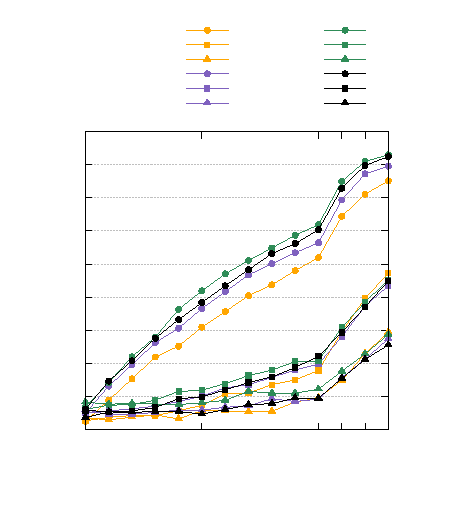
\includegraphics{../plots/strategies-acceptancerate}}%
    \gplfronttext
  \end{picture}%
\endgroup
 & % GNUPLOT: LaTeX picture with Postscript
\begingroup
\newcommand{\ft}[0]{\footnotesize}\newcommand{\ty}[0]{\tiny}
  \makeatletter
  \providecommand\color[2][]{%
    \GenericError{(gnuplot) \space\space\space\@spaces}{%
      Package color not loaded in conjunction with
      terminal option `colourtext'%
    }{See the gnuplot documentation for explanation.%
    }{Either use 'blacktext' in gnuplot or load the package
      color.sty in LaTeX.}%
    \renewcommand\color[2][]{}%
  }%
  \providecommand\includegraphics[2][]{%
    \GenericError{(gnuplot) \space\space\space\@spaces}{%
      Package graphicx or graphics not loaded%
    }{See the gnuplot documentation for explanation.%
    }{The gnuplot epslatex terminal needs graphicx.sty or graphics.sty.}%
    \renewcommand\includegraphics[2][]{}%
  }%
  \providecommand\rotatebox[2]{#2}%
  \@ifundefined{ifGPcolor}{%
    \newif\ifGPcolor
    \GPcolortrue
  }{}%
  \@ifundefined{ifGPblacktext}{%
    \newif\ifGPblacktext
    \GPblacktextfalse
  }{}%
  % define a \g@addto@macro without @ in the name:
  \let\gplgaddtomacro\g@addto@macro
  % define empty templates for all commands taking text:
  \gdef\gplbacktext{}%
  \gdef\gplfronttext{}%
  \makeatother
  \ifGPblacktext
    % no textcolor at all
    \def\colorrgb#1{}%
    \def\colorgray#1{}%
  \else
    % gray or color?
    \ifGPcolor
      \def\colorrgb#1{\color[rgb]{#1}}%
      \def\colorgray#1{\color[gray]{#1}}%
      \expandafter\def\csname LTw\endcsname{\color{white}}%
      \expandafter\def\csname LTb\endcsname{\color{black}}%
      \expandafter\def\csname LTa\endcsname{\color{black}}%
      \expandafter\def\csname LT0\endcsname{\color[rgb]{1,0,0}}%
      \expandafter\def\csname LT1\endcsname{\color[rgb]{0,1,0}}%
      \expandafter\def\csname LT2\endcsname{\color[rgb]{0,0,1}}%
      \expandafter\def\csname LT3\endcsname{\color[rgb]{1,0,1}}%
      \expandafter\def\csname LT4\endcsname{\color[rgb]{0,1,1}}%
      \expandafter\def\csname LT5\endcsname{\color[rgb]{1,1,0}}%
      \expandafter\def\csname LT6\endcsname{\color[rgb]{0,0,0}}%
      \expandafter\def\csname LT7\endcsname{\color[rgb]{1,0.3,0}}%
      \expandafter\def\csname LT8\endcsname{\color[rgb]{0.5,0.5,0.5}}%
    \else
      % gray
      \def\colorrgb#1{\color{black}}%
      \def\colorgray#1{\color[gray]{#1}}%
      \expandafter\def\csname LTw\endcsname{\color{white}}%
      \expandafter\def\csname LTb\endcsname{\color{black}}%
      \expandafter\def\csname LTa\endcsname{\color{black}}%
      \expandafter\def\csname LT0\endcsname{\color{black}}%
      \expandafter\def\csname LT1\endcsname{\color{black}}%
      \expandafter\def\csname LT2\endcsname{\color{black}}%
      \expandafter\def\csname LT3\endcsname{\color{black}}%
      \expandafter\def\csname LT4\endcsname{\color{black}}%
      \expandafter\def\csname LT5\endcsname{\color{black}}%
      \expandafter\def\csname LT6\endcsname{\color{black}}%
      \expandafter\def\csname LT7\endcsname{\color{black}}%
      \expandafter\def\csname LT8\endcsname{\color{black}}%
    \fi
  \fi
    \setlength{\unitlength}{0.0500bp}%
    \ifx\gptboxheight\undefined%
      \newlength{\gptboxheight}%
      \newlength{\gptboxwidth}%
      \newsavebox{\gptboxtext}%
    \fi%
    \setlength{\fboxrule}{0.5pt}%
    \setlength{\fboxsep}{1pt}%
\begin{picture}(3744.00,4608.00)%
    \gplgaddtomacro\gplbacktext{%
      \csname LTb\endcsname%
      \put(369,638){\makebox(0,0)[r]{\strut{}\ft 0.2}}%
      \csname LTb\endcsname%
      \put(369,1116){\makebox(0,0)[r]{\strut{}\ft 0.25}}%
      \csname LTb\endcsname%
      \put(369,1593){\makebox(0,0)[r]{\strut{}\ft 0.3}}%
      \csname LTb\endcsname%
      \put(369,2071){\makebox(0,0)[r]{\strut{}\ft 0.35}}%
      \csname LTb\endcsname%
      \put(369,2548){\makebox(0,0)[r]{\strut{}\ft 0.4}}%
      \csname LTb\endcsname%
      \put(369,3025){\makebox(0,0)[r]{\strut{}\ft 0.45}}%
      \csname LTb\endcsname%
      \put(369,3503){\makebox(0,0)[r]{\strut{}\ft 0.5}}%
      \put(501,418){\makebox(0,0){\strut{}\ft 0}}%
      \put(1571,418){\makebox(0,0){\strut{}\ft 0.1}}%
      \put(2640,418){\makebox(0,0){\strut{}\ft 0.2}}%
      \put(2854,418){\makebox(0,0){\strut{}}}%
      \put(3068,418){\makebox(0,0){\strut{}}}%
      \put(3282,418){\makebox(0,0){\strut{}\ft 0.5}}%
    }%
    \gplgaddtomacro\gplfronttext{%
      \csname LTb\endcsname%
      \put(-190,2070){\rotatebox{-270}{\makebox(0,0){\strut{}\ft Information rate}}}%
      \put(1891,154){\makebox(0,0){\strut{}\ft Attack probabilities}}%
      \csname LTb\endcsname%
      \put(1324,4475){\makebox(0,0)[r]{\strut{}\ty UC-DOR}}%
      \csname LTb\endcsname%
      \put(1324,4335){\makebox(0,0)[r]{\strut{}\ty G2C3}}%
      \csname LTb\endcsname%
      \put(1324,4195){\makebox(0,0)[r]{\strut{}\ty G2C4}}%
      \csname LTb\endcsname%
      \put(1324,4055){\makebox(0,0)[r]{\strut{}\ty UC-DM}}%
      \csname LTb\endcsname%
      \put(1324,3915){\makebox(0,0)[r]{\strut{}\ty G2C3}}%
      \csname LTb\endcsname%
      \put(1324,3775){\makebox(0,0)[r]{\strut{}\ty G2C4}}%
      \csname LTb\endcsname%
      \put(2647,4475){\makebox(0,0)[r]{\strut{}\ty UC-ROMM}}%
      \csname LTb\endcsname%
      \put(2647,4335){\makebox(0,0)[r]{\strut{}\ty G2C3}}%
      \csname LTb\endcsname%
      \put(2647,4195){\makebox(0,0)[r]{\strut{}\ty G2C4}}%
      \csname LTb\endcsname%
      \put(2647,4055){\makebox(0,0)[r]{\strut{}\ty UC-RAMM}}%
      \csname LTb\endcsname%
      \put(2647,3915){\makebox(0,0)[r]{\strut{}\ty G2C3}}%
      \csname LTb\endcsname%
      \put(2647,3775){\makebox(0,0)[r]{\strut{}\ty G2C4}}%
    }%
    \gplbacktext
    \put(0,0){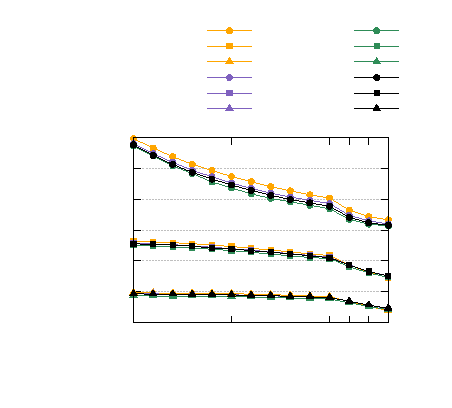
\includegraphics{../plots/strategies-informationrate}}%
    \gplfronttext
  \end{picture}%
\endgroup
 \\
        % GNUPLOT: LaTeX picture with Postscript
\begingroup
\newcommand{\ft}[0]{\footnotesize}\newcommand{\ty}[0]{\tiny}
  \makeatletter
  \providecommand\color[2][]{%
    \GenericError{(gnuplot) \space\space\space\@spaces}{%
      Package color not loaded in conjunction with
      terminal option `colourtext'%
    }{See the gnuplot documentation for explanation.%
    }{Either use 'blacktext' in gnuplot or load the package
      color.sty in LaTeX.}%
    \renewcommand\color[2][]{}%
  }%
  \providecommand\includegraphics[2][]{%
    \GenericError{(gnuplot) \space\space\space\@spaces}{%
      Package graphicx or graphics not loaded%
    }{See the gnuplot documentation for explanation.%
    }{The gnuplot epslatex terminal needs graphicx.sty or graphics.sty.}%
    \renewcommand\includegraphics[2][]{}%
  }%
  \providecommand\rotatebox[2]{#2}%
  \@ifundefined{ifGPcolor}{%
    \newif\ifGPcolor
    \GPcolortrue
  }{}%
  \@ifundefined{ifGPblacktext}{%
    \newif\ifGPblacktext
    \GPblacktextfalse
  }{}%
  % define a \g@addto@macro without @ in the name:
  \let\gplgaddtomacro\g@addto@macro
  % define empty templates for all commands taking text:
  \gdef\gplbacktext{}%
  \gdef\gplfronttext{}%
  \makeatother
  \ifGPblacktext
    % no textcolor at all
    \def\colorrgb#1{}%
    \def\colorgray#1{}%
  \else
    % gray or color?
    \ifGPcolor
      \def\colorrgb#1{\color[rgb]{#1}}%
      \def\colorgray#1{\color[gray]{#1}}%
      \expandafter\def\csname LTw\endcsname{\color{white}}%
      \expandafter\def\csname LTb\endcsname{\color{black}}%
      \expandafter\def\csname LTa\endcsname{\color{black}}%
      \expandafter\def\csname LT0\endcsname{\color[rgb]{1,0,0}}%
      \expandafter\def\csname LT1\endcsname{\color[rgb]{0,1,0}}%
      \expandafter\def\csname LT2\endcsname{\color[rgb]{0,0,1}}%
      \expandafter\def\csname LT3\endcsname{\color[rgb]{1,0,1}}%
      \expandafter\def\csname LT4\endcsname{\color[rgb]{0,1,1}}%
      \expandafter\def\csname LT5\endcsname{\color[rgb]{1,1,0}}%
      \expandafter\def\csname LT6\endcsname{\color[rgb]{0,0,0}}%
      \expandafter\def\csname LT7\endcsname{\color[rgb]{1,0.3,0}}%
      \expandafter\def\csname LT8\endcsname{\color[rgb]{0.5,0.5,0.5}}%
    \else
      % gray
      \def\colorrgb#1{\color{black}}%
      \def\colorgray#1{\color[gray]{#1}}%
      \expandafter\def\csname LTw\endcsname{\color{white}}%
      \expandafter\def\csname LTb\endcsname{\color{black}}%
      \expandafter\def\csname LTa\endcsname{\color{black}}%
      \expandafter\def\csname LT0\endcsname{\color{black}}%
      \expandafter\def\csname LT1\endcsname{\color{black}}%
      \expandafter\def\csname LT2\endcsname{\color{black}}%
      \expandafter\def\csname LT3\endcsname{\color{black}}%
      \expandafter\def\csname LT4\endcsname{\color{black}}%
      \expandafter\def\csname LT5\endcsname{\color{black}}%
      \expandafter\def\csname LT6\endcsname{\color{black}}%
      \expandafter\def\csname LT7\endcsname{\color{black}}%
      \expandafter\def\csname LT8\endcsname{\color{black}}%
    \fi
  \fi
    \setlength{\unitlength}{0.0500bp}%
    \ifx\gptboxheight\undefined%
      \newlength{\gptboxheight}%
      \newlength{\gptboxwidth}%
      \newsavebox{\gptboxtext}%
    \fi%
    \setlength{\fboxrule}{0.5pt}%
    \setlength{\fboxsep}{1pt}%
\begin{picture}(4030.00,3600.00)%
    \gplgaddtomacro\gplbacktext{%
      \csname LTb\endcsname%
      \put(858,660){\makebox(0,0)[r]{\strut{}\ty 0}}%
      \put(858,956){\makebox(0,0)[r]{\strut{}\ty 0.1}}%
      \put(858,1252){\makebox(0,0)[r]{\strut{}\ty 0.2}}%
      \put(858,1548){\makebox(0,0)[r]{\strut{}\ty 0.3}}%
      \put(858,1843){\makebox(0,0)[r]{\strut{}\ty 0.4}}%
      \put(858,2139){\makebox(0,0)[r]{\strut{}\ty 0.5}}%
      \put(858,2435){\makebox(0,0)[r]{\strut{}\ty 0.6}}%
      \put(990,440){\makebox(0,0){\strut{}\ty 0}}%
      \put(1982,440){\makebox(0,0){\strut{}\ty 0.1}}%
      \put(2973,440){\makebox(0,0){\strut{}\ty 0.2}}%
      \put(3171,440){\makebox(0,0){\strut{}}}%
      \put(3370,440){\makebox(0,0){\strut{}}}%
      \put(3568,440){\makebox(0,0){\strut{}\ty 0.5}}%
    }%
    \gplgaddtomacro\gplfronttext{%
      \csname LTb\endcsname%
      \put(352,1547){\rotatebox{-270}{\makebox(0,0){\strut{}\ft Residual error probability}}}%
      \put(2279,154){\makebox(0,0){\strut{}\ft Attack probabilities}}%
      \csname LTb\endcsname%
      \put(1676,3462){\makebox(0,0)[r]{\strut{}\ty UC-DOR}}%
      \csname LTb\endcsname%
      \put(1676,3312){\makebox(0,0)[r]{\strut{}\ty G2C3}}%
      \csname LTb\endcsname%
      \put(1676,3162){\makebox(0,0)[r]{\strut{}\ty G2C4}}%
      \csname LTb\endcsname%
      \put(1676,3012){\makebox(0,0)[r]{\strut{}\ty UC-DM}}%
      \csname LTb\endcsname%
      \put(1676,2862){\makebox(0,0)[r]{\strut{}\ty G2C3}}%
      \csname LTb\endcsname%
      \put(1676,2712){\makebox(0,0)[r]{\strut{}\ty UC-ROMM}}%
      \csname LTb\endcsname%
      \put(3089,3462){\makebox(0,0)[r]{\strut{}\ty G2C3}}%
      \csname LTb\endcsname%
      \put(3089,3312){\makebox(0,0)[r]{\strut{}\ty G2C4}}%
      \csname LTb\endcsname%
      \put(3089,3162){\makebox(0,0)[r]{\strut{}\ty UC-RAMM}}%
      \csname LTb\endcsname%
      \put(3089,3012){\makebox(0,0)[r]{\strut{}\ty G2C3}}%
      \csname LTb\endcsname%
      \put(3089,2862){\makebox(0,0)[r]{\strut{}\ty G2C4}}%
    }%
    \gplbacktext
    \put(0,0){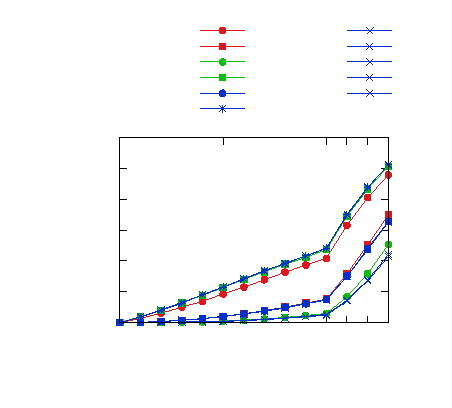
\includegraphics{../plots/strategies-residualerror}}%
    \gplfronttext
  \end{picture}%
\endgroup
 & % GNUPLOT: LaTeX picture with Postscript
\begingroup
\newcommand{\ft}[0]{\footnotesize}\newcommand{\ty}[0]{\tiny}
  \makeatletter
  \providecommand\color[2][]{%
    \GenericError{(gnuplot) \space\space\space\@spaces}{%
      Package color not loaded in conjunction with
      terminal option `colourtext'%
    }{See the gnuplot documentation for explanation.%
    }{Either use 'blacktext' in gnuplot or load the package
      color.sty in LaTeX.}%
    \renewcommand\color[2][]{}%
  }%
  \providecommand\includegraphics[2][]{%
    \GenericError{(gnuplot) \space\space\space\@spaces}{%
      Package graphicx or graphics not loaded%
    }{See the gnuplot documentation for explanation.%
    }{The gnuplot epslatex terminal needs graphicx.sty or graphics.sty.}%
    \renewcommand\includegraphics[2][]{}%
  }%
  \providecommand\rotatebox[2]{#2}%
  \@ifundefined{ifGPcolor}{%
    \newif\ifGPcolor
    \GPcolortrue
  }{}%
  \@ifundefined{ifGPblacktext}{%
    \newif\ifGPblacktext
    \GPblacktextfalse
  }{}%
  % define a \g@addto@macro without @ in the name:
  \let\gplgaddtomacro\g@addto@macro
  % define empty templates for all commands taking text:
  \gdef\gplbacktext{}%
  \gdef\gplfronttext{}%
  \makeatother
  \ifGPblacktext
    % no textcolor at all
    \def\colorrgb#1{}%
    \def\colorgray#1{}%
  \else
    % gray or color?
    \ifGPcolor
      \def\colorrgb#1{\color[rgb]{#1}}%
      \def\colorgray#1{\color[gray]{#1}}%
      \expandafter\def\csname LTw\endcsname{\color{white}}%
      \expandafter\def\csname LTb\endcsname{\color{black}}%
      \expandafter\def\csname LTa\endcsname{\color{black}}%
      \expandafter\def\csname LT0\endcsname{\color[rgb]{1,0,0}}%
      \expandafter\def\csname LT1\endcsname{\color[rgb]{0,1,0}}%
      \expandafter\def\csname LT2\endcsname{\color[rgb]{0,0,1}}%
      \expandafter\def\csname LT3\endcsname{\color[rgb]{1,0,1}}%
      \expandafter\def\csname LT4\endcsname{\color[rgb]{0,1,1}}%
      \expandafter\def\csname LT5\endcsname{\color[rgb]{1,1,0}}%
      \expandafter\def\csname LT6\endcsname{\color[rgb]{0,0,0}}%
      \expandafter\def\csname LT7\endcsname{\color[rgb]{1,0.3,0}}%
      \expandafter\def\csname LT8\endcsname{\color[rgb]{0.5,0.5,0.5}}%
    \else
      % gray
      \def\colorrgb#1{\color{black}}%
      \def\colorgray#1{\color[gray]{#1}}%
      \expandafter\def\csname LTw\endcsname{\color{white}}%
      \expandafter\def\csname LTb\endcsname{\color{black}}%
      \expandafter\def\csname LTa\endcsname{\color{black}}%
      \expandafter\def\csname LT0\endcsname{\color{black}}%
      \expandafter\def\csname LT1\endcsname{\color{black}}%
      \expandafter\def\csname LT2\endcsname{\color{black}}%
      \expandafter\def\csname LT3\endcsname{\color{black}}%
      \expandafter\def\csname LT4\endcsname{\color{black}}%
      \expandafter\def\csname LT5\endcsname{\color{black}}%
      \expandafter\def\csname LT6\endcsname{\color{black}}%
      \expandafter\def\csname LT7\endcsname{\color{black}}%
      \expandafter\def\csname LT8\endcsname{\color{black}}%
    \fi
  \fi
    \setlength{\unitlength}{0.0500bp}%
    \ifx\gptboxheight\undefined%
      \newlength{\gptboxheight}%
      \newlength{\gptboxwidth}%
      \newsavebox{\gptboxtext}%
    \fi%
    \setlength{\fboxrule}{0.5pt}%
    \setlength{\fboxsep}{1pt}%
\begin{picture}(4030.00,3600.00)%
    \gplgaddtomacro\gplbacktext{%
      \csname LTb\endcsname%
      \put(726,660){\makebox(0,0)[r]{\strut{}\ty 30}}%
      \csname LTb\endcsname%
      \put(726,1015){\makebox(0,0)[r]{\strut{}\ty 32}}%
      \csname LTb\endcsname%
      \put(726,1370){\makebox(0,0)[r]{\strut{}\ty 34}}%
      \csname LTb\endcsname%
      \put(726,1725){\makebox(0,0)[r]{\strut{}\ty 36}}%
      \csname LTb\endcsname%
      \put(726,2080){\makebox(0,0)[r]{\strut{}\ty 38}}%
      \csname LTb\endcsname%
      \put(726,2435){\makebox(0,0)[r]{\strut{}\ty 40}}%
      \put(858,440){\makebox(0,0){\strut{}\ty 0}}%
      \put(1900,440){\makebox(0,0){\strut{}\ty 0.1}}%
      \put(2943,440){\makebox(0,0){\strut{}\ty 0.2}}%
      \put(3151,440){\makebox(0,0){\strut{}}}%
      \put(3360,440){\makebox(0,0){\strut{}}}%
      \put(3568,440){\makebox(0,0){\strut{}\ty 0.5}}%
    }%
    \gplgaddtomacro\gplfronttext{%
      \csname LTb\endcsname%
      \put(352,1547){\rotatebox{-270}{\makebox(0,0){\strut{}\ft Avg. end-to-end latency in cycles}}}%
      \put(2213,154){\makebox(0,0){\strut{}\ft Attack probabilities}}%
      \csname LTb\endcsname%
      \put(1610,3462){\makebox(0,0)[r]{\strut{}\ty UC-DOR}}%
      \csname LTb\endcsname%
      \put(1610,3312){\makebox(0,0)[r]{\strut{}\ty G2C3}}%
      \csname LTb\endcsname%
      \put(1610,3162){\makebox(0,0)[r]{\strut{}\ty G2C4}}%
      \csname LTb\endcsname%
      \put(1610,3012){\makebox(0,0)[r]{\strut{}\ty UC-DM}}%
      \csname LTb\endcsname%
      \put(1610,2862){\makebox(0,0)[r]{\strut{}\ty G2C3}}%
      \csname LTb\endcsname%
      \put(1610,2712){\makebox(0,0)[r]{\strut{}\ty G2C4}}%
      \csname LTb\endcsname%
      \put(3023,3462){\makebox(0,0)[r]{\strut{}\ty UC-ROMM}}%
      \csname LTb\endcsname%
      \put(3023,3312){\makebox(0,0)[r]{\strut{}\ty G2C3}}%
      \csname LTb\endcsname%
      \put(3023,3162){\makebox(0,0)[r]{\strut{}\ty G2C4}}%
      \csname LTb\endcsname%
      \put(3023,3012){\makebox(0,0)[r]{\strut{}\ty UC-RAMM}}%
      \csname LTb\endcsname%
      \put(3023,2862){\makebox(0,0)[r]{\strut{}\ty G2C3}}%
      \csname LTb\endcsname%
      \put(3023,2712){\makebox(0,0)[r]{\strut{}\ty G2C4}}%
    }%
    \gplbacktext
    \put(0,0){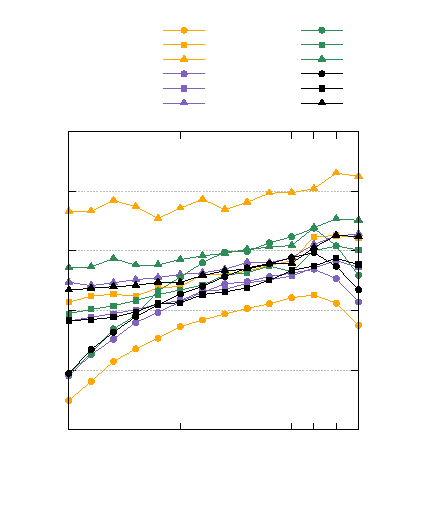
\includegraphics{../plots/strategies-endtoendlatency}}%
    \gplfronttext
  \end{picture}%
\endgroup

    \end{tabular}
    \caption[Results for routing strategies experiment]{long}
    \label{fig:resultsroutingstratsexperiment}
\end{figure}

% Heatmap of router workload
\begin{figure}
    \begin{tabular}{cc}
        % GNUPLOT: LaTeX picture with Postscript
\begingroup
\newcommand{\ft}[0]{\footnotesize}\newcommand{\ty}[0]{\tiny}
  \makeatletter
  \providecommand\color[2][]{%
    \GenericError{(gnuplot) \space\space\space\@spaces}{%
      Package color not loaded in conjunction with
      terminal option `colourtext'%
    }{See the gnuplot documentation for explanation.%
    }{Either use 'blacktext' in gnuplot or load the package
      color.sty in LaTeX.}%
    \renewcommand\color[2][]{}%
  }%
  \providecommand\includegraphics[2][]{%
    \GenericError{(gnuplot) \space\space\space\@spaces}{%
      Package graphicx or graphics not loaded%
    }{See the gnuplot documentation for explanation.%
    }{The gnuplot epslatex terminal needs graphicx.sty or graphics.sty.}%
    \renewcommand\includegraphics[2][]{}%
  }%
  \providecommand\rotatebox[2]{#2}%
  \@ifundefined{ifGPcolor}{%
    \newif\ifGPcolor
    \GPcolortrue
  }{}%
  \@ifundefined{ifGPblacktext}{%
    \newif\ifGPblacktext
    \GPblacktextfalse
  }{}%
  % define a \g@addto@macro without @ in the name:
  \let\gplgaddtomacro\g@addto@macro
  % define empty templates for all commands taking text:
  \gdef\gplbacktext{}%
  \gdef\gplfronttext{}%
  \makeatother
  \ifGPblacktext
    % no textcolor at all
    \def\colorrgb#1{}%
    \def\colorgray#1{}%
  \else
    % gray or color?
    \ifGPcolor
      \def\colorrgb#1{\color[rgb]{#1}}%
      \def\colorgray#1{\color[gray]{#1}}%
      \expandafter\def\csname LTw\endcsname{\color{white}}%
      \expandafter\def\csname LTb\endcsname{\color{black}}%
      \expandafter\def\csname LTa\endcsname{\color{black}}%
      \expandafter\def\csname LT0\endcsname{\color[rgb]{1,0,0}}%
      \expandafter\def\csname LT1\endcsname{\color[rgb]{0,1,0}}%
      \expandafter\def\csname LT2\endcsname{\color[rgb]{0,0,1}}%
      \expandafter\def\csname LT3\endcsname{\color[rgb]{1,0,1}}%
      \expandafter\def\csname LT4\endcsname{\color[rgb]{0,1,1}}%
      \expandafter\def\csname LT5\endcsname{\color[rgb]{1,1,0}}%
      \expandafter\def\csname LT6\endcsname{\color[rgb]{0,0,0}}%
      \expandafter\def\csname LT7\endcsname{\color[rgb]{1,0.3,0}}%
      \expandafter\def\csname LT8\endcsname{\color[rgb]{0.5,0.5,0.5}}%
    \else
      % gray
      \def\colorrgb#1{\color{black}}%
      \def\colorgray#1{\color[gray]{#1}}%
      \expandafter\def\csname LTw\endcsname{\color{white}}%
      \expandafter\def\csname LTb\endcsname{\color{black}}%
      \expandafter\def\csname LTa\endcsname{\color{black}}%
      \expandafter\def\csname LT0\endcsname{\color{black}}%
      \expandafter\def\csname LT1\endcsname{\color{black}}%
      \expandafter\def\csname LT2\endcsname{\color{black}}%
      \expandafter\def\csname LT3\endcsname{\color{black}}%
      \expandafter\def\csname LT4\endcsname{\color{black}}%
      \expandafter\def\csname LT5\endcsname{\color{black}}%
      \expandafter\def\csname LT6\endcsname{\color{black}}%
      \expandafter\def\csname LT7\endcsname{\color{black}}%
      \expandafter\def\csname LT8\endcsname{\color{black}}%
    \fi
  \fi
    \setlength{\unitlength}{0.0500bp}%
    \ifx\gptboxheight\undefined%
      \newlength{\gptboxheight}%
      \newlength{\gptboxwidth}%
      \newsavebox{\gptboxtext}%
    \fi%
    \setlength{\fboxrule}{0.5pt}%
    \setlength{\fboxsep}{1pt}%
\begin{picture}(1440.00,1440.00)%
    \gplgaddtomacro\gplbacktext{%
    }%
    \gplgaddtomacro\gplfronttext{%
    }%
    \gplbacktext
    \put(0,0){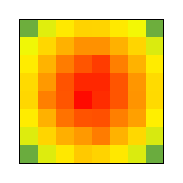
\includegraphics{../plots/heatmap-iwa-g2c3-dor}}%
    \gplfronttext
  \end{picture}%
\endgroup
 & % GNUPLOT: LaTeX picture with Postscript
\begingroup
\newcommand{\ft}[0]{\footnotesize}\newcommand{\ty}[0]{\tiny}
  \makeatletter
  \providecommand\color[2][]{%
    \GenericError{(gnuplot) \space\space\space\@spaces}{%
      Package color not loaded in conjunction with
      terminal option `colourtext'%
    }{See the gnuplot documentation for explanation.%
    }{Either use 'blacktext' in gnuplot or load the package
      color.sty in LaTeX.}%
    \renewcommand\color[2][]{}%
  }%
  \providecommand\includegraphics[2][]{%
    \GenericError{(gnuplot) \space\space\space\@spaces}{%
      Package graphicx or graphics not loaded%
    }{See the gnuplot documentation for explanation.%
    }{The gnuplot epslatex terminal needs graphicx.sty or graphics.sty.}%
    \renewcommand\includegraphics[2][]{}%
  }%
  \providecommand\rotatebox[2]{#2}%
  \@ifundefined{ifGPcolor}{%
    \newif\ifGPcolor
    \GPcolortrue
  }{}%
  \@ifundefined{ifGPblacktext}{%
    \newif\ifGPblacktext
    \GPblacktextfalse
  }{}%
  % define a \g@addto@macro without @ in the name:
  \let\gplgaddtomacro\g@addto@macro
  % define empty templates for all commands taking text:
  \gdef\gplbacktext{}%
  \gdef\gplfronttext{}%
  \makeatother
  \ifGPblacktext
    % no textcolor at all
    \def\colorrgb#1{}%
    \def\colorgray#1{}%
  \else
    % gray or color?
    \ifGPcolor
      \def\colorrgb#1{\color[rgb]{#1}}%
      \def\colorgray#1{\color[gray]{#1}}%
      \expandafter\def\csname LTw\endcsname{\color{white}}%
      \expandafter\def\csname LTb\endcsname{\color{black}}%
      \expandafter\def\csname LTa\endcsname{\color{black}}%
      \expandafter\def\csname LT0\endcsname{\color[rgb]{1,0,0}}%
      \expandafter\def\csname LT1\endcsname{\color[rgb]{0,1,0}}%
      \expandafter\def\csname LT2\endcsname{\color[rgb]{0,0,1}}%
      \expandafter\def\csname LT3\endcsname{\color[rgb]{1,0,1}}%
      \expandafter\def\csname LT4\endcsname{\color[rgb]{0,1,1}}%
      \expandafter\def\csname LT5\endcsname{\color[rgb]{1,1,0}}%
      \expandafter\def\csname LT6\endcsname{\color[rgb]{0,0,0}}%
      \expandafter\def\csname LT7\endcsname{\color[rgb]{1,0.3,0}}%
      \expandafter\def\csname LT8\endcsname{\color[rgb]{0.5,0.5,0.5}}%
    \else
      % gray
      \def\colorrgb#1{\color{black}}%
      \def\colorgray#1{\color[gray]{#1}}%
      \expandafter\def\csname LTw\endcsname{\color{white}}%
      \expandafter\def\csname LTb\endcsname{\color{black}}%
      \expandafter\def\csname LTa\endcsname{\color{black}}%
      \expandafter\def\csname LT0\endcsname{\color{black}}%
      \expandafter\def\csname LT1\endcsname{\color{black}}%
      \expandafter\def\csname LT2\endcsname{\color{black}}%
      \expandafter\def\csname LT3\endcsname{\color{black}}%
      \expandafter\def\csname LT4\endcsname{\color{black}}%
      \expandafter\def\csname LT5\endcsname{\color{black}}%
      \expandafter\def\csname LT6\endcsname{\color{black}}%
      \expandafter\def\csname LT7\endcsname{\color{black}}%
      \expandafter\def\csname LT8\endcsname{\color{black}}%
    \fi
  \fi
    \setlength{\unitlength}{0.0500bp}%
    \ifx\gptboxheight\undefined%
      \newlength{\gptboxheight}%
      \newlength{\gptboxwidth}%
      \newsavebox{\gptboxtext}%
    \fi%
    \setlength{\fboxrule}{0.5pt}%
    \setlength{\fboxsep}{1pt}%
\begin{picture}(1440.00,1440.00)%
    \gplgaddtomacro\gplbacktext{%
    }%
    \gplgaddtomacro\gplfronttext{%
    }%
    \gplbacktext
    \put(0,0){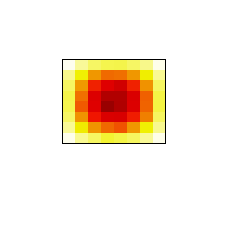
\includegraphics{../plots/heatmap-iwa-g2c3-dm}}%
    \gplfronttext
  \end{picture}%
\endgroup
 \\
        (a) & (b) \\
        % GNUPLOT: LaTeX picture with Postscript
\begingroup
\newcommand{\ft}[0]{\footnotesize}\newcommand{\st}[0]{\scriptsize}
  \makeatletter
  \providecommand\color[2][]{%
    \GenericError{(gnuplot) \space\space\space\@spaces}{%
      Package color not loaded in conjunction with
      terminal option `colourtext'%
    }{See the gnuplot documentation for explanation.%
    }{Either use 'blacktext' in gnuplot or load the package
      color.sty in LaTeX.}%
    \renewcommand\color[2][]{}%
  }%
  \providecommand\includegraphics[2][]{%
    \GenericError{(gnuplot) \space\space\space\@spaces}{%
      Package graphicx or graphics not loaded%
    }{See the gnuplot documentation for explanation.%
    }{The gnuplot epslatex terminal needs graphicx.sty or graphics.sty.}%
    \renewcommand\includegraphics[2][]{}%
  }%
  \providecommand\rotatebox[2]{#2}%
  \@ifundefined{ifGPcolor}{%
    \newif\ifGPcolor
    \GPcolortrue
  }{}%
  \@ifundefined{ifGPblacktext}{%
    \newif\ifGPblacktext
    \GPblacktextfalse
  }{}%
  % define a \g@addto@macro without @ in the name:
  \let\gplgaddtomacro\g@addto@macro
  % define empty templates for all commands taking text:
  \gdef\gplbacktext{}%
  \gdef\gplfronttext{}%
  \makeatother
  \ifGPblacktext
    % no textcolor at all
    \def\colorrgb#1{}%
    \def\colorgray#1{}%
  \else
    % gray or color?
    \ifGPcolor
      \def\colorrgb#1{\color[rgb]{#1}}%
      \def\colorgray#1{\color[gray]{#1}}%
      \expandafter\def\csname LTw\endcsname{\color{white}}%
      \expandafter\def\csname LTb\endcsname{\color{black}}%
      \expandafter\def\csname LTa\endcsname{\color{black}}%
      \expandafter\def\csname LT0\endcsname{\color[rgb]{1,0,0}}%
      \expandafter\def\csname LT1\endcsname{\color[rgb]{0,1,0}}%
      \expandafter\def\csname LT2\endcsname{\color[rgb]{0,0,1}}%
      \expandafter\def\csname LT3\endcsname{\color[rgb]{1,0,1}}%
      \expandafter\def\csname LT4\endcsname{\color[rgb]{0,1,1}}%
      \expandafter\def\csname LT5\endcsname{\color[rgb]{1,1,0}}%
      \expandafter\def\csname LT6\endcsname{\color[rgb]{0,0,0}}%
      \expandafter\def\csname LT7\endcsname{\color[rgb]{1,0.3,0}}%
      \expandafter\def\csname LT8\endcsname{\color[rgb]{0.5,0.5,0.5}}%
    \else
      % gray
      \def\colorrgb#1{\color{black}}%
      \def\colorgray#1{\color[gray]{#1}}%
      \expandafter\def\csname LTw\endcsname{\color{white}}%
      \expandafter\def\csname LTb\endcsname{\color{black}}%
      \expandafter\def\csname LTa\endcsname{\color{black}}%
      \expandafter\def\csname LT0\endcsname{\color{black}}%
      \expandafter\def\csname LT1\endcsname{\color{black}}%
      \expandafter\def\csname LT2\endcsname{\color{black}}%
      \expandafter\def\csname LT3\endcsname{\color{black}}%
      \expandafter\def\csname LT4\endcsname{\color{black}}%
      \expandafter\def\csname LT5\endcsname{\color{black}}%
      \expandafter\def\csname LT6\endcsname{\color{black}}%
      \expandafter\def\csname LT7\endcsname{\color{black}}%
      \expandafter\def\csname LT8\endcsname{\color{black}}%
    \fi
  \fi
    \setlength{\unitlength}{0.0500bp}%
    \ifx\gptboxheight\undefined%
      \newlength{\gptboxheight}%
      \newlength{\gptboxwidth}%
      \newsavebox{\gptboxtext}%
    \fi%
    \setlength{\fboxrule}{0.5pt}%
    \setlength{\fboxsep}{1pt}%
\begin{picture}(1872.00,1872.00)%
    \gplgaddtomacro\gplbacktext{%
    }%
    \gplgaddtomacro\gplfronttext{%
    }%
    \gplbacktext
    \put(0,0){
\includegraphics{../plots/heatmap-iwa-g2c3-romm}}%
    \gplfronttext
  \end{picture}%
\endgroup
 & % GNUPLOT: LaTeX picture with Postscript
\begingroup
\newcommand{\ft}[0]{\footnotesize}\newcommand{\st}[0]{\scriptsize}
  \makeatletter
  \providecommand\color[2][]{%
    \GenericError{(gnuplot) \space\space\space\@spaces}{%
      Package color not loaded in conjunction with
      terminal option `colourtext'%
    }{See the gnuplot documentation for explanation.%
    }{Either use 'blacktext' in gnuplot or load the package
      color.sty in LaTeX.}%
    \renewcommand\color[2][]{}%
  }%
  \providecommand\includegraphics[2][]{%
    \GenericError{(gnuplot) \space\space\space\@spaces}{%
      Package graphicx or graphics not loaded%
    }{See the gnuplot documentation for explanation.%
    }{The gnuplot epslatex terminal needs graphicx.sty or graphics.sty.}%
    \renewcommand\includegraphics[2][]{}%
  }%
  \providecommand\rotatebox[2]{#2}%
  \@ifundefined{ifGPcolor}{%
    \newif\ifGPcolor
    \GPcolortrue
  }{}%
  \@ifundefined{ifGPblacktext}{%
    \newif\ifGPblacktext
    \GPblacktextfalse
  }{}%
  % define a \g@addto@macro without @ in the name:
  \let\gplgaddtomacro\g@addto@macro
  % define empty templates for all commands taking text:
  \gdef\gplbacktext{}%
  \gdef\gplfronttext{}%
  \makeatother
  \ifGPblacktext
    % no textcolor at all
    \def\colorrgb#1{}%
    \def\colorgray#1{}%
  \else
    % gray or color?
    \ifGPcolor
      \def\colorrgb#1{\color[rgb]{#1}}%
      \def\colorgray#1{\color[gray]{#1}}%
      \expandafter\def\csname LTw\endcsname{\color{white}}%
      \expandafter\def\csname LTb\endcsname{\color{black}}%
      \expandafter\def\csname LTa\endcsname{\color{black}}%
      \expandafter\def\csname LT0\endcsname{\color[rgb]{1,0,0}}%
      \expandafter\def\csname LT1\endcsname{\color[rgb]{0,1,0}}%
      \expandafter\def\csname LT2\endcsname{\color[rgb]{0,0,1}}%
      \expandafter\def\csname LT3\endcsname{\color[rgb]{1,0,1}}%
      \expandafter\def\csname LT4\endcsname{\color[rgb]{0,1,1}}%
      \expandafter\def\csname LT5\endcsname{\color[rgb]{1,1,0}}%
      \expandafter\def\csname LT6\endcsname{\color[rgb]{0,0,0}}%
      \expandafter\def\csname LT7\endcsname{\color[rgb]{1,0.3,0}}%
      \expandafter\def\csname LT8\endcsname{\color[rgb]{0.5,0.5,0.5}}%
    \else
      % gray
      \def\colorrgb#1{\color{black}}%
      \def\colorgray#1{\color[gray]{#1}}%
      \expandafter\def\csname LTw\endcsname{\color{white}}%
      \expandafter\def\csname LTb\endcsname{\color{black}}%
      \expandafter\def\csname LTa\endcsname{\color{black}}%
      \expandafter\def\csname LT0\endcsname{\color{black}}%
      \expandafter\def\csname LT1\endcsname{\color{black}}%
      \expandafter\def\csname LT2\endcsname{\color{black}}%
      \expandafter\def\csname LT3\endcsname{\color{black}}%
      \expandafter\def\csname LT4\endcsname{\color{black}}%
      \expandafter\def\csname LT5\endcsname{\color{black}}%
      \expandafter\def\csname LT6\endcsname{\color{black}}%
      \expandafter\def\csname LT7\endcsname{\color{black}}%
      \expandafter\def\csname LT8\endcsname{\color{black}}%
    \fi
  \fi
    \setlength{\unitlength}{0.0500bp}%
    \ifx\gptboxheight\undefined%
      \newlength{\gptboxheight}%
      \newlength{\gptboxwidth}%
      \newsavebox{\gptboxtext}%
    \fi%
    \setlength{\fboxrule}{0.5pt}%
    \setlength{\fboxsep}{1pt}%
\begin{picture}(1872.00,1872.00)%
    \gplgaddtomacro\gplbacktext{%
    }%
    \gplgaddtomacro\gplfronttext{%
      \csname LTb\endcsname%
      \put(1638,644){\makebox(0,0)[l]{\strut{}\st 20000}}%
      \put(1638,804){\makebox(0,0)[l]{\strut{}\st 40000}}%
      \put(1638,965){\makebox(0,0)[l]{\strut{}\st 60000}}%
      \put(1638,1126){\makebox(0,0)[l]{\strut{}\st 80000}}%
      \put(1638,1287){\makebox(0,0)[l]{\strut{}\st 100000}}%
      \put(1638,1448){\makebox(0,0)[l]{\strut{}\st 120000}}%
      \put(2760,1046){\rotatebox{-270}{\makebox(0,0){\strut{}\ft Flits forwarded}}}%
    }%
    \gplbacktext
    \put(0,0){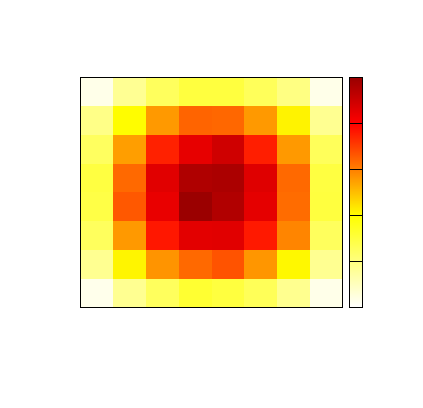
\includegraphics{../plots/heatmap-iwa-g2c3-ramm}}%
    \gplfronttext
  \end{picture}%
\endgroup
 \\
        (c) & (d) \\
    \end{tabular}
    \caption[Heatmaps of the routers for different routing strategies]{Heatmaps of the routers for different routing strategies.}
    \label{fig:resultsroutingstratheatmaps}
\end{figure}

\subsection{Increased ARQ limit}

\section{Area Overhead}
Encryption units: 3x PRINCE (8260 GE each\footnote{For Nangate 45 nm Generic technology with a unit delay of 1000. Both lower and higher values were
obtained with other technologies.} \cite[16]{borghoff12prince})

Authentication units: 9x PRINCE (8260 GE each)

Network coding lookup tables: 7080 GEs (G2C3) or 16992 GEs (G2C4) \cite[5]{moriam18activeattackers}

compare with the area overhead estimated by moriam et al., also reference the state-of-the-art MPSoC [14]

\iffalse
"Results for IWA-NC confirm the alleged positive effect of NC in unreliable networks"

"Creation rate adjustment to keep the base injection rate constant is reflected in the differing information rates"

"IDA: 4 flits need to arrive unharmed for successful transmission unit, 3 for FGA, and 2 for IWA"

"NC proves to provide a performance improvement, although more in the sense of less residual errors than a decrease in latency since ARQs are still
limited to 1 per transmission unit across all variants."
\fi
